\RequirePackage[OT1]{fontenc}
\documentclass[10pt,journal]{IEEEtran}
\usepackage{graphicx,amsmath,amssymb,booktabs,array,url}
\usepackage[nocompress]{cite}
\interdisplaylinepenalty=2500
\usepackage[colorlinks=true,allcolors=blue]{hyperref}

\newcounter{algorithm}
\renewcommand{\thealgorithm}{\arabic{algorithm}}
\makeatletter
\newcommand{\fps@algorithm}{tbp}
\newcommand{\ftype@algorithm}{1}
\newcommand{\ext@algorithm}{loa}
\newcommand{\fnum@algorithm}{Algorithm~\thealgorithm}
% Local ruled algorithm caption; leave IEEE table/figure captions untouched.
\newenvironment{algorithm}[1][t]{\@float{algorithm}[#1]%
  \long\def\@makecaption##1##2{%
    \par\hrule height .8pt\kern2pt
    {\normalfont\normalsize\noindent\textbf{##1:} ##2\par}%
    \kern2pt\hrule height .8pt\kern2pt}%
}{\end@float}
\makeatother
\newcommand{\ARC}{ARC-Audit}
\newcounter{proposition}
\newenvironment{proposition}[1]{%
  \refstepcounter{proposition}\par\smallskip\noindent
  \textbf{Proposition~\theproposition\ (#1). }\ignorespaces
}{\par\smallskip}
\newenvironment{claimproof}{\par\noindent\emph{Proof. }\ignorespaces
}{\hfill\textit{Q.E.D.}\par\smallskip}
\newcounter{algline}
\newcommand{\al}{\stepcounter{algline}\thealgline:}
\newcommand{\tabnote}[1]{\par\smallskip\parbox{\linewidth}{\footnotesize #1}}
\title{ARC-Audit: Dependency-Aware Auditing\\and Authenticated Record Recovery\\for Industrial IoT Data}
\author{Anonymous Author(s)}
\begin{document}
\bstctlcite{IEEEexample:BSTcontrol}
\maketitle
\begin{abstract}
Shared compression reduces storage for industrial Internet of Things (IIoT) data, yet couples single-record decoding to shared dictionary pages. Because encryption hides which dictionary rows a record references, a public verifier without the decryption key and an authorized retriever with the key require different page sets for the same record. ARC-Audit resolves this asymmetry through a single authenticated layout mapping logical bit spans to ciphertext pages. The public verifier constructs an authenticated recovery closure (ARC) covering all potential dependencies, merges overlapping pages across targets, and issues a fresh aggregate challenge. By contrast, the authorized retriever authenticates and decrypts reference pages first to resolve exact dictionary rows before fetching remaining pages. Within a per-batch storage budget, ARC-Audit protects selected ciphertext pages via Reed--Solomon coding and enforces identical integrity checks on directly fetched and repaired objects. This paper proves decoding correctness, closure coverage, equal-leakage confidentiality, and response and record authenticity. On two full segments of the HAI dataset (442,802 records), ARC-Audit cuts sealed cloud storage by 35.5\%--53.2\% relative to EntroGD and GreedyGD, cuts online audit traffic by 39$\times$--69$\times$ relative to MPA and Miao without a gigabyte-scale external directory, and under 5\% erasures increases recovery by +4.0/+3.6 percentage points via exact retrieval ($\beta{=}0.10$) while reaching 72.4\%/76.4\% at $1.26\times$ storage (outperforming TREAT at $1.29\times$ and RepEC-Core at $1.59$--$1.60\times$).
\end{abstract}
\begin{IEEEkeywords}
Industrial Internet of Things, generalized deduplication, public integrity
auditing, authenticated record recovery, dependency closure, authenticated encryption.
\end{IEEEkeywords}

\section{Introduction}\label{sec:introduction}
\IEEEPARstart{O}{utsourced} industrial Internet of Things (IIoT) archives must support both public integrity auditing and reliable record recovery. Shared compression reduces storage by exploiting repetition across sensor fields and records. For example, generalized deduplication (GD) represents data blocks using shared bases paired with record-specific references and deviations~\cite{Talasila2019}, and secure similarity-based deduplication has been applied to outsourced IIoT storage~\cite{Gao2024}. However, sharing introduces cross-object decoding dependencies: reconstructing a single record requires both record-specific objects and shared dictionary pages, all of which must be authenticated against the requested data version.

When dictionary references are encrypted, public verifiers and authorized retrievers face an inherent information asymmetry and select different page sets for the same record. Lacking decryption keys, a public verifier relies solely on the authenticated layout and must include complete dictionaries for the relevant groups to cover every row a record could reference. An authorized retriever can instead decrypt the references and fetch only the dictionary pages actually identified. Consequently, when an unreferenced dictionary page is lost, full public coverage fails even though the record itself remains decodable.

Prior work optimizes each piece of this pipeline in isolation: compression methods refine the underlying representation~\cite{Hurst2024GreedyGD}, public storage proofs authenticate responses over challenged objects~\cite{ShachamWaters2013}, selective access systems optimize query retrieval~\cite{Taurone2024TREAT}, and shared-storage protection mitigates the loss of common chunks~\cite{Bhagwat2006Reliability}. What connects these problems is determining which ciphertext pages suffice to decode a requested record under the information available to each role, and binding those pages to a single authenticated version.

ARC-Audit introduces an \emph{authenticated recovery closure} (ARC) to unify dependency selection across both roles over one compressed batch. The data owner publishes a signed layout mapping logical bit spans to ciphertext pages while keeping all decoding content encrypted. The public verifier uses this layout to collect the relevant group dictionaries, merge overlapping pages across targets, and bind the resulting closure to a fresh aggregate challenge. The authorized retriever first authenticates and decrypts the reference pages to resolve the exact dependencies before fetching the remaining objects. Within a per-batch storage budget, ARC-Audit applies Reed--Solomon (RS) coding to selected ciphertext pages, checks repaired and directly fetched pages under the same integrity rules, and accepts records only after complete deterministic decoding.

The main contributions of this paper are summarized as follows.
\begin{itemize}
\item \emph{Dual-role dependency planning over an encrypted layout.} This paper designs a single authenticated layout that separates structural bit-span geometry from encrypted decoding values. This enables a public verifier to form a sufficient closure without decryption keys while allowing an authorized retriever to narrow retrieval to exact dependencies after authenticating references.
\item \emph{Dependency-aware public aggregate auditing.} ARC-Audit couples closure planning with a BLS12-381 linear homomorphic authenticator that merges overlapping pages across targets and binds the snapshot, targets, and selected page set to a fresh challenge, avoiding both reference transfer and per-page proof overhead.
\item \emph{Addressable shared representation and budgeted exact recovery.} ARC-Audit's grouped generalized deduplication encoder (SDA-GGD) confirms field merges against full-input serialized cost while preserving page-level span boundaries. For recovery under erasures, a ciphertext RS layer protects selected pages within a serialized storage cap and verifies repaired pages identically to direct fetches.
\end{itemize}

This paper evaluates ARC-Audit on both segments of the HAI 21.03 industrial control dataset against internal ablations and eight published deduplication, auditing, and recovery schemes. Across seven daily batches, SDA-GGD cuts sealed cloud storage by 10.8\%--11.4\% over per-field GD and 35.5\%--53.2\% over EntroGD and GreedyGD while accelerating end-to-end sealing by 47.9\%--62.8\%. Public aggregation eliminates first-stage reference transfer and gigabyte-scale external directories while cutting online audit traffic by 39$\times$--69$\times$ relative to MPA and Miao. Under 5\% nominal erasures, exact dependency resolution adds +4.0/+3.6 percentage points over conservative closure retrieval at $\beta{=}0.10$, and full-coverage ARC-Audit ($1.26\times$) outperforms TREAT ($1.29\times$) by 47.6--56.8 percentage points and RepEC-Core ($1.59$--$1.60\times$) by 12.4--13.2 percentage points.
\section{Related Work}
\subsection{Shared Compression and Selective Access}
Shared compression partitions record content between local encodings and shared dictionaries. GD reconstructs data chunks from shared bases and per-record deviations~\cite{Talasila2019}. Building on this model, GreedyGD selects base bits to support both compression and direct analytics~\cite{Hurst2024GreedyGD}, while EntroGD integrates analytical summaries with entropy-guided compression~\cite{Zhao2026EntroGD}. Whereas these schemes focus on storage reduction and in-place analytics, ARC-Audit bridges shared representations and cryptographic verification through authenticated record spans and dictionary geometry, enabling ciphertext page selection before reading references.

Confidentiality and selective access impose additional constraints on shared representations. Secure similarity deduplication addresses ownership and confidentiality via fuzzy message-locked encryption with ownership proofs~\cite{Jiang2023FuzzyDedup} and outsourced IIoT storage management~\cite{Gao2024}. Closer to the ARC-Audit access model, TREAT combines GD, coding, rearrangement, and selective fetching for distributed IoT queries~\cite{Taurone2024TREAT}. Its GD representation supports BaseID-addressed dictionary entries, and its evaluated query pipeline fetches the dictionary upfront and uses BaseIDs for predicate filtering. In contrast, ARC-Audit operates over a single authenticated layout across two distinct roles: a public verifier covers all potential decoding dependencies while references remain encrypted, whereas an authorized retriever authenticates both the references and the resulting ciphertext dependencies before accepting a canonical record.

\subsection{Public Auditing and Retrievability}
Public storage verification establishes integrity guarantees over challenged objects. Provable data possession (PDP) verifies outsourced storage~\cite{Ateniese2007PDP}, and proofs of retrievability (PoR) link challenge responses to data recovery via extraction~\cite{Juels2007POR,ShachamWaters2013}. Subsequent work extends PoR frameworks~\cite{Bowers2009PORTheory}, pairs integrity checking with distributed redundancy in HAIL~\cite{Bowers2009HAIL}, and supports updates via authenticated dictionaries in dynamic PDP~\cite{Erway2009DPDP}. Recent compressed PDP constructions reduce authenticator storage and employ proof exchange with linear communication for decentralized multi-cloud self-auditing~\cite{Yang2025CompressedPDP}. Rather than challenging arbitrary blocks or entire files, ARC-Audit derives the challenged page set directly from a record's decoding dependencies.

Shared-data auditing also lowers authentication redundancy and supports selective verification. Earlier schemes integrate auditing and deduplication using proofs of storage with deduplication~\cite{Zheng2012POSD}, shared authenticators~\cite{Tian2022SharedAudit}, client-side off-chain deduplication~\cite{Zhang2023BlockchainAudit}, and reduced key and authenticator redundancy~\cite{Miao2024SharedAudit}. Privacy-preserving variants protect file ownership during encrypted deduplication and auditing~\cite{Song2023EncryptedAudit} or safeguard file-tag and audit-proof privacy alongside identity-based broadcast encryption~\cite{Zhang2025PrivacyAudit}. Fine-grained deduplication further connects auditing to retrieval: Liu et al. deduplicate ciphertexts and authentication tags within and across users and employ a reconstruction matrix and Bloom filter for distributed block retrieval~\cite{Liu2025FineGrained}, FiDD pairs fine-grained deduplication with dynamic public auditing~\cite{Huang2026FiDD}, while searchable auditing with arbitration~\cite{Miao2025}, dynamic mixed auditing~\cite{Pan2026}, and updatable multi-copy authentication~\cite{Xu2026MPA} address selective verification in other shared settings.

Authenticated data structures bind directory responses to source-authenticated commitments~\cite{Goodrich2003ADS}. ARC-Audit extends this principle to shared-compressed record decoding: the public verifier validates the signed layout before selecting a sufficient closure, while authorized recovery authenticates reference pages before resolving dictionary rows via BaseIDs.

\subsection{Reliability of Shared Storage}
Protecting shared storage requires accounting for the records that depend on each object, because losing a common chunk impairs multiple logical records. Prior studies establish this dependency effect through loss-impact-based replication~\cite{Bhagwat2006Reliability} and reliability analysis of deduplicated, erasure-coded storage~\cite{Li2010Reliability}. System designs such as CDStore coordinate reliability, security, and storage efficiency across multiple clouds by combining convergent dispersal with two-stage deduplication~\cite{Li2015CDStore}, Li et al. combine non-systematic Cauchy ramp secret sharing with deduplication for decentralized cloud storage~\cite{Li2024TNSE}, Per-File Parity integrates pre-deduplication parity with intra- and inter-file recovery~\cite{Wu2019PFP}, and RepEC+ coordinates replication, erasure coding, selection, and cooperative restore~\cite{Zuo2022RepECPlus}. ARC-Audit applies standard RS coding~\cite{ReedSolomon1960} over complete ciphertext pages and holds the code and storage budget fixed while evaluating how protection placement and exact dependency selection affect authenticated record recovery. Table~\ref{tab:lit-compare} summarizes the capability coverage of the related schemes evaluated or contrasted in Section~\ref{sec:eval}.

\begin{table*}[t]\centering\scriptsize
\caption{QUALITATIVE COMPARISON OF RELATED DEDUPLICATION, AUDITING, AND RECOVERY SCHEMES}\label{tab:lit-compare}
\setlength{\tabcolsep}{2.8pt}
\begin{tabular}{@{}lcccccc@{}}\toprule
Scheme & Multi-Field Dedup & Public Keyless Audit & Exact Dep.\ Binding & Selective Local Recovery & Active Tamper Resist. & Extra Storage / Ratio\\\midrule
GreedyGD~\cite{Hurst2024GreedyGD} & Greedy GD & $\times$ (no tags) & Plaintext only & Analytic slices & $\times$ & Base GD\\
EntroGD~\cite{Zhao2026EntroGD} & Entropy GD & $\times$ (no tags) & Plaintext only & Analytic slices & $\times$ & Base GD\\
FiDD~\cite{Huang2026FiDD} & Fine-grained (adapt.) & $\checkmark$ (Type-III) & Owner dir. & $\times$ (audit only) & $\checkmark$ (pairing) & Static tags + dir.\\
Miao~\cite{Miao2025} & Keyword-indexed & $\checkmark$ (Type-III) & Inverted index & Unblinded owner & $\checkmark$ (pairing) & Index + blinded\\
MPA~\cite{Xu2026MPA} & Single-copy (adapt.) & $\checkmark$ (KZG+Merkle) & Owner dir. & $\times$ (audit only) & $\checkmark$ (KZG+Merkle) & SRS + Merkle + dir.\\
TREAT~\cite{Taurone2024TREAT} & Static batch RLNC & $\times$ & Fixed batch & $\checkmark$ (RLNC 4/5) & Hash-pinned & $\sim 1.29\times$\\
RepEC+~\cite{Zuo2022RepECPlus} & Overlap-aware RCF & $\times$ & Owner dir. & $\checkmark$ (Rep.+RS) & Hash-pinned & $\sim 1.59$--$1.60\times$\\
Li2024~\cite{Li2024TNSE} & Ramp SS ($t{=}1,k{=}4,n{=}6$) & $\times$ & Per-page shares & $\checkmark$ (4-of-6) & Share digests & $\sim 2.18\times$\\
PFP~\cite{Wu2019PFP} & Cross-file parity & $\times$ & Cross-file & Cross-file & Parity check & Qualitative only\\
\textbf{ARC-Audit (This paper)} & \textbf{SDA-GGD} & \textbf{$\checkmark$ (Public closure)} & \textbf{$\checkmark$ (Manifest+exact)} & \textbf{$\checkmark$ (RS+exact)} & \textbf{$\checkmark$ (AEAD+BLS+RS)} & \textbf{$1.10\times$ / $1.26\times$}\\\bottomrule
\end{tabular}
\tabnote{Quantitative evaluations in Section~\ref{sec:eval} implement component-level cryptographic/coding adapters over shared encrypted archives; blockchain consensus, dynamic updates, and multi-user key-exchange layers of external systems are excluded and noted per baseline. PFP uses cross-file overlapping parity and is compared qualitatively.}
\end{table*}

\section{System Model and Problem Formulation}\label{sec:model}
\subsection{System Roles and Trusted State}
Fig.~\ref{fig:architecture} illustrates the four system roles over an immutable batch snapshot and target set $T$. The \emph{owner} encodes and encrypts each batch, generates public audit tags, signs a canonical manifest, and retains the batch-scoped base catalog and private encoding state. The \emph{cloud service provider} (CSP) stores ciphertext pages, tags, public parameters, the signed layout, and any deployed protection sidecar, answering audit challenges and object fetches.

Both clients pin the owner's verification key and expected manifest digest. The \emph{public verifier} authenticates the layout and parameters to issue keyless audits, whereas the \emph{authorized retriever} also holds the batch decryption key to recover canonical records. The signed manifest binds the batch identifier, layout, page descriptors (identities, valid lengths, SHA-256 digests), protocol version, and audit parameters; clients retain the manifest, whose size scales with the page count. Encryption, manifest signing, and audit tagging use independent secrets, and cross-batch requests execute per batch under each batch's pins and cryptographic context.

\subsection{Records and Page Dependencies}
Each canonical record contains scaled process values, an index, timestamp, and schema-declared labels. For batch $b$, the logical container $F$ is partitioned into plaintext slices $F_p$ of at most $P_0$ bytes, each sealed into a ciphertext \emph{page} $C_p$ with identity $(b,p)\in\mathcal P$. The authenticated public layout $\mathcal L$ maps any logical bit interval $[a,a+w)$ to its intersecting pages:
\begin{equation}\label{eq:phi}
\Phi_{\mathcal L}(a,w)=
\left\{(b,p):\left\lfloor\frac{a}{8P_0}\right\rfloor
\leq p\leq\left\lfloor\frac{a+w-1}{8P_0}\right\rfloor\right\},
\end{equation}
with $\Phi_{\mathcal L}(a,0)=\varnothing$.

Under a fixed representation and deterministic decoder, record $i$'s exact dependency set $\mathcal D_{\mathcal L}(i)$ contains the pages carrying private structure, references, local data, labels, and its actually referenced dictionary rows. Because references are encrypted, the public recovery closure $K_{\mathcal L}(i)$ includes the complete dictionaries of the relevant groups to cover every possible reference:
\begin{equation}\label{eq:sufficient-set}
\mathcal D_{\mathcal L}(i)\subseteq K_{\mathcal L}(i)\subseteq\mathcal P.
\end{equation}
For target set $T$, let $U(T)=\bigcup_{i\in T}K_{\mathcal L}(i)$ and $D(T)=\bigcup_{i\in T}\mathcal D_{\mathcal L}(i)$, so $D(T)\subseteq U(T)$. The verifier computes $U(T)$ directly from $\mathcal L$, whereas the retriever authenticates and decrypts reference pages to resolve $D(T)$ (omitting subscript $\mathcal L$ when clear).

\subsection{Threat Model and Public View}
The owner and clients follow the protocol with authentic pins and keys. The untrusted CSP may observe public state and requests, omit objects, corrupt ciphertexts, substitute metadata or tags, or replay stale snapshots and responses. The pinned manifest digest fixes the snapshot, a fresh challenge binds each audit response, and manifest integrity relies on signature unforgeability and hash collision resistance.

The public view exposes record counts, page lengths, associated data, group and bit geometry, dictionary cardinalities, visible protection layouts, and public audit targets and page sets, while constants, timestamps, labels, references, bases, and deviations remain encrypted. If a deployment exposes authorized recovery page-access traces, those traces enter its leakage profile because they depend on private references. Section~\ref{sec:security} formalizes equal-leakage confidentiality under standard key-derivation and AEAD assumptions.

\subsection{Audit, Recovery, and Protection Goals}
\emph{Public audit.} For targets $T$, the verifier authenticates the manifest, challenges $U(T)$, and accepts only if every involved batch's aggregate response verifies under the fresh challenge context.

\emph{Authorized recovery.} Let $\mathcal A$ denote the pages whose committed ciphertext and authenticated plaintext are obtained directly or via verified repair. Decoding $\widehat r_i$ against canonical record $r_i$ succeeds iff
\begin{equation}\label{eq:record-recovery}
\mathsf{Rec}_i(\mathcal A)=
\mathbf1\{\mathcal D_{\mathcal L}(i)\subseteq\mathcal A
\ \land\ \widehat r_i=r_i\}.
\end{equation}
The retriever checks input authenticity and complete decoding, returning all requested records or $\bot$.

\emph{Budgeted protection.} Because multiple records share dictionary pages, ARC-Audit allocates ciphertext redundancy within a per-batch fraction $\beta$ of stored ciphertext bytes (Section~\ref{sec:protection}) to maximize record survival under erasures.

\begin{table}[t]\centering\small
\caption{NOTATION FOR ARC-AUDIT}\label{tab:notation}
\begin{tabular}{@{}l>{\raggedright\arraybackslash}p{.70\columnwidth}@{}}\toprule
Symbol & Meaning\\\midrule
$b$, $b_T$ & Batch identity; number of batches involved in $T$\\
$F,F_p,C_p$ & Logical container, plaintext slice, ciphertext object\\
$k_b,N_p,A_p$ & Batch encryption key, nonce, associated data\\
$\mathcal L,\Phi_{\mathcal L}$ & Authenticated public layout and bit-span map\\
$\ell(p),\tau_p$ & Valid ciphertext length and public audit tag\\
$\mathcal D(i),K(i)$ & Exact dependencies and public sufficient closure\\
$D(T),U(T)$ & Exact dependency union and audit closure union\\
$\pi=(\sigma,\boldsymbol\mu)$ & Aggregate audit response\\
$\beta,B_{\rm side}$ & Protection budget fraction and charged sidecar bytes\\\bottomrule
\end{tabular}\end{table}

\begin{figure*}[t]\centering
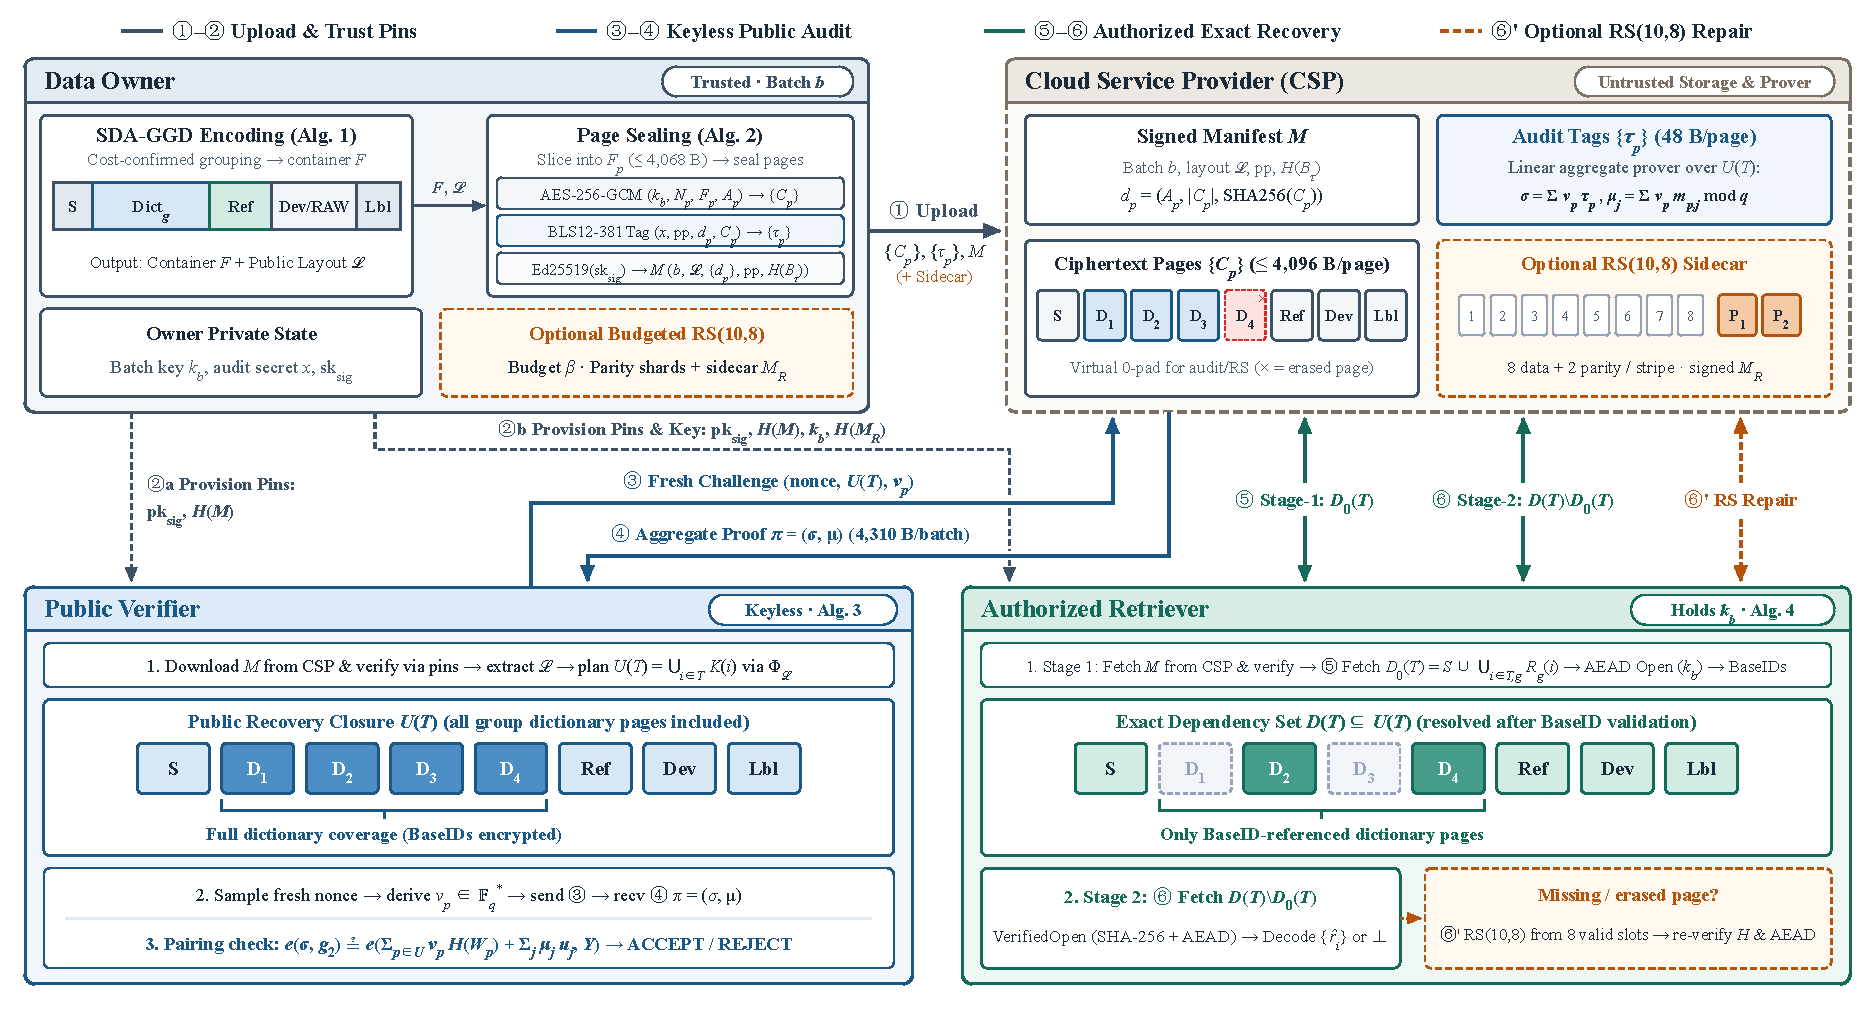
\includegraphics[width=\textwidth]{figures/architecture.pdf}
\caption{ARC-Audit system architecture. The page strips illustrate dictionary coverage for public auditing and authorized recovery.}
\label{fig:architecture}\end{figure*}

\section{ARC-Audit Design}\label{sec:design}
\subsection{Overview}
As shown in Fig.~\ref{fig:architecture}, ARC-Audit coordinates encoding, sealing, auditing, recovery, and budgeted protection around one authenticated layout. Section~\ref{sec:c1} introduces SDA-GGD, which groups fields under full-input serialized cost confirmation, and Section~\ref{sec:seal} seals the logical container into addressable ciphertext pages committed by a signed manifest. Sections~\ref{sec:c2}--\ref{sec:audit} then derive the public closure $U(T)$ and fresh BLS12-381 aggregate audits, while Sections~\ref{sec:c3}--\ref{sec:protection} resolve exact dependencies $D(T)$ and verify RS-repaired ciphertext pages under identical integrity rules.

\subsection{Cost-Confirmed Shared Representation}\label{sec:c1}
SDA-GGD partitions nonconstant fields into groups (storing constants once) to shrink serialized size while preserving page-addressable span geometry. For a group $G$ of width $L_g$ bits with $k$ base-bit positions and $M_g$ distinct bases, each record stores a $b_g=\lceil\log_2 M_g\rceil$-bit BaseID and an $(L_g-k)$-bit deviation, while a group dictionary stores the $M_g$ bases. Across $n$ records, the independently byte-rounded serialized group cost is
\begin{equation}\label{eq:cost}
\begin{split}
C(G)={}&C_{\mathrm{hdr}}(G,k)+\lceil M_gk/8\rceil+\lceil nb_g/8\rceil\\
 &+\lceil n(L_g-k)/8\rceil,
\end{split}
\end{equation}
where $C_{\mathrm{hdr}}(G,k)=11+2|G|+2k$ bytes encodes the mode, field IDs, and base-bit positions, and a RAW fallback costs $C_{\mathrm{hdr}}(G,0)+\lceil nL_g/8\rceil$. The container cost is $C_0+\sum_G C(G)$, where $C_0$ covers fixed schema, constants, time/label streams, and the global header.

\emph{Within-group configuration.}
$\operatorname{Config}(X,G)$ stably sorts the bits of $G$ by increasing empirical binary entropy (preserving field-concatenation order on ties) and scans prefixes $k=0,\ldots,L_g$ until $M_g=n$. A prefix is feasible under dependency cap $\rho\in(0,1]$ if $R_{\mathrm{dep}}=\max_v n_v/n\leq\rho$, where $n_v$ counts records sharing base $v$. The configurator chooses the lowest-cost feasible prefix (breaking ties by smaller $k$, or minimizing $R_{\mathrm{dep}}$ if none is feasible) and falls back to RAW whenever RAW cost is no larger.

\emph{Sample-ranked, full-data-confirmed grouping.}
Algorithm~\ref{alg:grouping} initializes one singleton group per nonconstant field and prioritizes candidate pairs $(G_a,G_b)$ by sampled byte gain $\widehat\Delta=C_m(G_a)+C_m(G_b)-C_m(G_a\mathbin{\|}G_b)$ over fixed sample indices $I$ ($\|$ denotes ordered field concatenation). Before any merge, $\operatorname{Config}(X,G_a\mathbin{\|}G_b)$ re-evaluates exact full-input serialized gain $\Delta_{\mathrm{full}}=C(G_a)+C(G_b)-C(G_c;c)$ and headerless payload gain $\Delta_P$, accepting only when both $\Delta_{\mathrm{full}}>0$ and $\Delta_P>0$. To handle refreshed priorities without stalling, Algorithm~\ref{alg:grouping} tracks rejected versioned pairs in $J$, discards stale endpoints, and caps candidate deferrals at $d_{\max}=8$ against queue-head gain $\operatorname{TopGain}(Q)$. Because every accepted merge strictly decreases both $C$ and $C_{\mathrm{pay}}$ while reducing the active-group count by one, starting from $g_0$ groups accepts at most $g_0-1$ merges and terminates finitely. Final cloud bytes (Eq.~\eqref{eq:cloud-cost}) additionally include encryption framing, audit tags, and the manifest.

\begin{algorithm}[t]\centering\normalsize\setcounter{algline}{0}
\caption{Cost-Confirmed Grouping.}\label{alg:grouping}
\begin{tabular}{@{}r@{\enspace} >{\raggedright\arraybackslash}p{.88\columnwidth}@{}}
\multicolumn{2}{@{}p{\columnwidth}@{}}{\textbf{Require:} Records $X$, schema $\Sigma$, sample indices $I$.}\\
\multicolumn{2}{@{}p{\columnwidth}@{}}{\textbf{Ensure:} Logical container $F$ and public layout $\mathcal L$.}\\
\al & $\mathcal G\gets$ singleton nonconstant-field groups.\\
\al & Configure $\mathcal G$ on $X$ and $X_I$; $J\gets\varnothing$.\\
\al & $Q\gets$ positive sampled-gain pairs; initialize $d_e=0$.\\
\al & \textbf{while} $Q\neq\varnothing$ \textbf{do}\\
\al & \hspace*{1em}$e=(G_a,G_b,\text{versions})\gets\operatorname{PopMax}(Q)$.\\
\al & \hspace*{1em}\textbf{if} $e$ is stale or $e\in J$, \textbf{continue}.\\
\al & \hspace*{1em}$(\widehat\Delta,\widehat c)\gets\operatorname{SampleGain}(X_I,G_a,G_b)$.\\
\al & \hspace*{1em}\textbf{if} $\widehat\Delta\leq0$, add $e$ to $J$; \textbf{continue}.\\
\al & \hspace*{1em}\textbf{if} $\operatorname{TopGain}(Q)>\widehat\Delta$ and $d_e<d_{\max}$ \textbf{then}\\
\al & \hspace*{2em}$d_e\gets d_e+1$; requeue $e$ with $\widehat\Delta$; \textbf{continue}.\\
\al & \hspace*{1em}\textbf{end if}\\
\al & \hspace*{1em}$G_c\gets G_a\mathbin{\|}G_b$; $c\gets\operatorname{Config}(X,G_c)$.\\
\al & \hspace*{1em}$\Delta_{\mathrm{full}}\gets C(G_a)+C(G_b)-C(G_c;c)$.\\
\al & \hspace*{1em}$\Delta_P\gets C_{\mathrm{pay}}(G_a)+C_{\mathrm{pay}}(G_b)-C_{\mathrm{pay}}(G_c;c)$.\\
\al & \hspace*{1em}\textbf{if} $\Delta_{\mathrm{full}}>0$ and $\Delta_P>0$ \textbf{then}\\
\al & \hspace*{2em}Replace $G_a,G_b$ in $\mathcal G$ by $G_c$ with $(c,\widehat c)$.\\
\al & \hspace*{2em}Invalidate old-group entries; queue positive new/live pairs.\\
\al & \hspace*{1em}\textbf{else} add $e$ to $J$.\\
\al & \hspace*{1em}\textbf{end if}\\
\al & \textbf{end while}\\
\al & $(F,\mathcal L)\gets\operatorname{Serialize}(X,\Sigma,\mathcal G)$.\\
\al & \textbf{return} $(F,\mathcal L)$.\\\bottomrule
\end{tabular}
\end{algorithm}

\subsection{Page Encryption and Authenticated Layout}\label{sec:seal}
To decouple dependency geometry from private values, the public layout $\mathcal L$ records stream offsets, widths, modes, base-bit positions, dictionary cardinalities, and record counts for Eq.~\eqref{eq:phi}, while the private header, constants, and encoded streams remain inside the encrypted slices of $F$.

For each batch (Algorithm~\ref{alg:seal}), the owner samples a 256-bit batch identifier $b$ and random master secret, derives $k_b$ via HKDF-SHA256 with salt $b$ and context \texttt{ARC/ENC/v1}~\cite{RFC5869}, and seals each slice $F_p$ ($P_0=4{,}068$ B) under AES-256-GCM~\cite{RFC5116} using the 96-bit page index $N_p$ as a unique nonce and canonical associated data $A_p$ (binding protocol, owner domain, batch, page ID, codec, and plaintext length):
\begin{equation}\label{eq:cipher}
C_p=N_p\,\|\,\mathsf{Enc}_{k_b}(N_p,F_p,A_p).
\end{equation}
The 12-byte nonce and 16-byte tag yield valid length $\ell(p)=|F_p|+28\leq4{,}096$ B (virtual zero padding for auditing/repair adds no stored bytes), giving $N=\lceil B_F/P_0\rceil$ pages and $B_{\rm cipher}=B_F+28N$ bytes for container size $B_F>0$. Each descriptor $d_p$ records $(A_p,|C_p|,\mathsf{SHA256}(C_p))$ and is bound into the page's audit tag. The owner then serializes all tags in ascending page order and Ed25519-signs the canonical manifest $M$ committing $\{d_p\}$, $\mathcal L$, public audit parameters, and $\mathsf{SHA256}(B_\tau)$ without circular digests, provisioning the 32-byte public key and $\mathsf{SHA256}(M)$ as client pins.

\begin{algorithm}[t]\centering\normalsize\setcounter{algline}{0}
\caption{Seal a Data Batch.}\label{alg:seal}
\begin{tabular}{@{}r@{\enspace} >{\raggedright\arraybackslash}p{.88\columnwidth}@{}}
\multicolumn{2}{@{}p{\columnwidth}@{}}{\textbf{Require:} Logical container $F$, public layout $\mathcal L$, owner domain.}\\
\multicolumn{2}{@{}p{\columnwidth}@{}}{\textbf{Ensure:} Ciphertext objects, audit tags, signed manifest, and client pins.}\\
\al & Sample fresh batch $b$ and encryption master secret; derive $k_b$.\\
\al & Generate independent audit secret $x$, public parameters $\mathsf{pp}$, and a manifest signing key.\\
\al & \textbf{for each} slice $F_p$ of at most 4,068 B \textbf{do}\\
\al & \hspace*{1em}$N_p\gets\operatorname{Encode}_{96}(p)$; form associated data $A_p$.\\
\al & \hspace*{1em}$C_p\gets N_p\|\mathsf{Enc}_{k_b}(N_p,F_p,A_p)$.\\
\al & \hspace*{1em}$d_p\gets(A_p,|C_p|,\mathsf{SHA256}(C_p))$.\\
\al & \hspace*{1em}$\tau_p\gets\operatorname{Tag}(x,\mathsf{pp},d_p,C_p)$.\\
\al & \textbf{end for}\\
\al & Serialize tags in page-index order to obtain $B_\tau$.\\
\al & $M\gets\operatorname{Manifest}(b,\mathcal L,\{d_p\},\mathsf{pp},\mathsf{SHA256}(B_\tau))$.\\
\al & Sign canonical $M$; provision signing public key and $\mathsf{SHA256}(M)$ as pins.\\
\al & Retain batch-scoped private encoding state and decryption capability.\\
\al & \textbf{return} $\{C_p\},\{\tau_p\},M$, signature, and pins.\\\bottomrule
\end{tabular}\end{algorithm}

\subsection{Authenticated Recovery Closure}\label{sec:c2}
Under $\Phi_{\mathcal L}$, let $S$, $R_g(i)$, $V_g(i)$, and $L(i)$ denote the pages intersecting private structural metadata, record $i$'s reference span in group $g$, its deviation/RAW span, and its label bits, and let $\mathcal P_g^{\rm dict}$ cover group $g$'s complete dictionary (empty for RAW groups). The single-record public recovery closure is
\begin{equation}\label{eq:closure}
K(i)=S\cup L(i)\cup\bigcup_g
\bigl(R_g(i)\cup V_g(i)\cup\mathcal P_g^{\rm dict}\bigr),
\end{equation}
which covers any valid BaseID without decryption. An authorized retriever instead authenticates and decrypts $S$ and $R_g(i)$, validates each BaseID, and replaces $\mathcal P_g^{\rm dict}$ with only the referenced dictionary-row pages to obtain $\mathcal D(i)$. Across a target set $T$, union planning merges overlaps into $U(T)=\bigcup_{i\in T}K(i)$ (separately per batch for cross-batch queries), reducing uncached read bytes $B_N$ to $B_U$:
\begin{equation}\label{eq:reads}
B_U=\sum_{p\in U(T)}\ell(p),\qquad
B_N=\sum_{i\in T}\sum_{p\in K(i)}\ell(p).
\end{equation}

\subsection{Fresh Public Aggregate Audit}\label{sec:audit}
Public-Aggregate verifies a linear response over $U(T)$ bound to a fresh challenge (Algorithm~\ref{alg:audit}). Each page $C_p$ is virtually zero-padded to $s=133$ little-endian 31-byte sectors satisfying $m_{p,j}<2^{248}<q$ for BLS12-381 order $q$, covering nonce, ciphertext, and AEAD tag while signed valid lengths control tail removal. Following Shacham--Waters~\cite{ShachamWaters2013}, the owner picks secret $x$, publishes $Y=xg_2$, and computes tags in $\mathbb G_1$ under $e:\mathbb G_1\times\mathbb G_2\to\mathbb G_T$ using domain-separated hash-to-curve~\cite{RFC9380} bases $u_j$ and descriptor hash $H(W_p)$ (binding $d_p$ and the parameter fingerprint):
\begin{equation}\label{eq:tag}
\tau_p=x\left(H(W_p)+\sum_{j=1}^{s}m_{p,j}u_j\right).
\end{equation}

For each batch request, the verifier samples a fresh 256-bit nonce, binds snapshot, parameters, $T_b$, $U_b$, policy, and session into a canonical challenge digest, and expands nonzero weights $\nu_p\in\mathbb F_q^*$ via SHA-512 with retry on zero. The CSP reads each unique $p\in U$ and returns
\begin{equation}\label{eq:aggregate}
\sigma=\sum_{p\in U}\nu_p\tau_p,\qquad
\mu_j=\sum_{p\in U}\nu_pm_{p,j}\pmod q.
\end{equation}
After context, framing, point, subgroup, and scalar-range validation (excluding identity bases), the verifier checks
\begin{equation}\label{eq:pairing}
e(\sigma,g_2)=e\left(\sum_{p\in U}\nu_pH(W_p)+\sum_j\mu_ju_j,Y\right).
\end{equation}

\begin{algorithm}[t]\centering\normalsize\setcounter{algline}{0}
\caption{ARC-Audit Public Closure Audit.}\label{alg:audit}
\begin{tabular}{@{}r@{\enspace} >{\raggedright\arraybackslash}p{.88\columnwidth}@{}}
\multicolumn{2}{@{}p{\columnwidth}@{}}{\textbf{Require:} Targets $T$, corresponding manifests and pins, public audit parameters.}\\
\multicolumn{2}{@{}p{\columnwidth}@{}}{\textbf{Ensure:} \texttt{ACCEPT} or \texttt{REJECT}.}\\
\al & \textbf{if} $T=\varnothing$, \textbf{return} \texttt{REJECT}. Partition $T$ into per-batch sets $\{T_b\}$.\\
\al & \textbf{for each} involved batch $b$ \textbf{do}\\
\al & \hspace*{1em}Authenticate its manifest against the pins. Check target ranges, uniqueness, and public parameters.\\
\al & \hspace*{1em}\textbf{if} validation fails, \textbf{return} \texttt{REJECT}.\\
\al & \hspace*{1em}$U_b\gets\operatorname{SortUnique}(\bigcup_{i\in T_b}K_{\mathcal L_b}(i))$.\\
\al & \hspace*{1em}Sample fresh nonce; bind expected snapshot, request, $T_b$, and $U_b$.\\
\al & \hspace*{1em}Derive $\nu_p\in\mathbb F_q^*$ for $p\in U_b$; send challenge and retain expected context.\\
\al & \hspace*{1em}CSP reads unique $C_p$ and uses $\tau_p$ for $p\in U_b$ to respond by Eq.~\eqref{eq:aggregate}.\\
\al & \hspace*{1em}Verifier checks framing, context, encodings, and Eq.~\eqref{eq:pairing}.\\
\al & \hspace*{1em}\textbf{if} the response is missing or any check fails, \textbf{return} \texttt{REJECT}.\\
\al & \textbf{end for}\\
\al & \textbf{return} \texttt{ACCEPT}.\\\bottomrule
\end{tabular}\end{algorithm}

Each serialized aggregate proof occupies $4+2+48+133\cdot32=4{,}310$ B per batch ($4{,}310b_T$ B across $b_T$ batches, compared with $4{,}318u$ B for unaggregated per-page proofs over $u$ pages under the same challenge).

\subsection{Authenticated Exact Record Recovery}\label{sec:c3}
Algorithm~\ref{alg:recovery} executes two-stage exact recovery (Exact) per batch using the helper $\operatorname{VerifiedOpen}(p)$, which fetches $C_p$ directly or via verified erasure repair, checks its committed descriptor and digest, performs AEAD decryption, and caches verified ciphertexts and plaintexts for intra-request reuse. Stage~1 opens the structural and reference pages $D_0(T)$ to validate BaseIDs and form $D(T)$. Stage~2 then opens only the remaining dependencies in $D(T)\setminus\operatorname{dom}(\mathcal C)$ before checking framing consistency against $\mathcal L$ and deterministically decoding $\{\widehat r_i\}_{i\in T}$ (returning $\bot$ on any verification or decoding error). The Conservative baseline replaces $D_0(T)$ with $U(T)$ in line~3 while preserving identical verification and decoding.

\begin{algorithm}[t]\centering\normalsize\setcounter{algline}{0}
\caption{Authenticated Exact Record Recovery.}\label{alg:recovery}
\begin{tabular}{@{}r@{\enspace} >{\raggedright\arraybackslash}p{.88\columnwidth}@{}}
\multicolumn{2}{@{}p{\columnwidth}@{}}{\textbf{Require:} Manifest and pins, decryption capability, targets $T$, cloud fetch interface, and optionally a signed sidecar with its provisioned public key and digest.}\\
\multicolumn{2}{@{}p{\columnwidth}@{}}{\textbf{Ensure:} Complete decoded records $\{\widehat r_i\}_{i\in T}$ or $\bot$.}\\
\al & Authenticate the manifest and validate $T$. If present, authenticate the sidecar against its own pin and check its binding to the batch snapshot.\\
\al & \textbf{if} validation fails, \textbf{return} $\bot$.\\
\al & $D_0(T)\gets S\cup\bigcup_{i\in T,g}R_g(i)$; $\mathcal C\gets\varnothing$.\\
\al & \textbf{for each} $p\in D_0(T)$ \textbf{do}\\
\al & \hspace*{1em}$\mathcal C[p]\gets\operatorname{VerifiedOpen}(p)$; on failure \textbf{return} $\bot$.\\
\al & \textbf{end for}\\
\al & Parse the authenticated private structure and BaseIDs.\\
\al & \textbf{if} parsing fails or any BaseID is out of range, \textbf{return} $\bot$.\\
\al & Form $D(T)$ by adding to $D_0(T)$ the pages covering target deviations or RAW data, labels, and the dictionary rows selected by the validated BaseIDs.\\
\al & \textbf{for each} $p\in D(T)\setminus\operatorname{dom}(\mathcal C)$ \textbf{do}\\
\al & \hspace*{1em}$\mathcal C[p]\gets\operatorname{VerifiedOpen}(p)$; on failure \textbf{return} $\bot$.\\
\al & \textbf{end for}\\
\al & Check private/public framing and decode from $\mathcal C$.\\
\al & \textbf{if} framing or complete decoding fails, \textbf{return} $\bot$.\\
\al & \textbf{return} $\{\widehat r_i\}_{i\in T}$.\\\bottomrule
\end{tabular}\end{algorithm}

\subsection{Budgeted Ciphertext Protection}\label{sec:protection}
A systematic RS$(10,8)$ sidecar over GF$(256)$ groups eight ciphertext pages per stripe and stores two 4,096-byte parity shards (leaving original ciphertexts intact, virtually zero-padding short pages to 4,096 B, and declaring virtual zero slots for partial stripes). Parity covers complete ciphertexts including nonces and AEAD tags, and a signed sidecar binds the parent snapshot, stripe membership, and parity digests.

Given a per-batch budget fraction $\beta$, protection policies (Dictionary, Uniform, FrequencyD) rank pages into a common admitted stripe count $s_R$ satisfying
\begin{equation}\label{eq:budget}
B_{\rm side,b}=8{,}192s_R+|M_R|+128\leq\left\lfloor\beta B_{\rm cipher,b}\right\rfloor,
\end{equation}
where $|M_R|$ is the serialized sidecar manifest and 128 B accounts for its signature, public key, and digest pin. When an original page is missing during $\operatorname{VerifiedOpen}$, the retriever authenticates available stripe shards against committed digests, counts declared virtual zero slots, reconstructs the page via RS$(10,8)$ from any eight distinct valid slots, truncates to $\ell(p)$, and checks both the original SHA-256 digest and AEAD tag before caching.

\subsection{Computation and Storage Accounting}\label{sec:accounting}
For a batch of $N$ pages and $u=|U(T)|$ challenged pages, closure union runs in $O(\sum_{i\in T}|K(i)|)$ expected time with $O(u)$ state. Tagging processes $Ns$ sectors, proving accumulates $us$ scalar products and $u$ weighted tags, and verification computes $u$ descriptor hashes, $s$ sector-base terms, and two pairings (summing across involved batches). Without a protection sidecar, sealed cloud storage is
\begin{equation}\label{eq:cloud-cost}
B_{\rm cloud}=B_{\rm cipher}+B_{\rm tags}+B_{\rm manifest},
\end{equation}
where $B_{\rm cipher}=B_F+28N$ (AEAD framing), $B_{\rm tags}=48N$, and $B_{\rm manifest}$ includes public parameters. Owner-side private state and deployed sidecar bytes are accounted separately.

\section{Security and Recoverability Analysis}\label{sec:security}
Let $C_p$ and $F_p$ denote the genuine ciphertext and plaintext slice of page $p$ in the expected snapshot under the model in Section~\ref{sec:model}.

\subsection{Representation Correctness and Closure Coverage}\label{sec:representation-proof}\label{sec:closure-proof}
\begin{proposition}{Correct decoding and closure coverage}\label{prop:representation}\label{prop:closure}
For a correctly constructed batch, the original dependency pages suffice to decode the target records, and $D(T)\subseteq U(T)$ for every valid target set $T$.
\end{proposition}
\begin{claimproof}
For record $i$ and GD group $g$ with base-bit positions $I_g$ and complement $J_g$, the encoder writes $x_{i,g}[I_g]=B_{g,\mathrm{ID}_{i,g}}$ and $x_{i,g}[J_g]=d_{i,g}$. Reassembling complementary positions, reversing exact decimal scaling, and reading RAW, constant, timestamp, and label fields deterministically reconstructs $r_i$. Moreover, each referenced dictionary row interval satisfies $L_{g,\mathrm{ID}_{i,g}}\subseteq L_g^{\mathrm{dict}}$, so $\Phi_{\mathcal L}(L_{g,\mathrm{ID}_{i,g}})\subseteq\Phi_{\mathcal L}(L_g^{\mathrm{dict}})$; since both policies include identical structure, reference, local-data, and label pages, taking unions over groups and targets yields $\mathcal D_{\mathcal L}(i)\subseteq K_{\mathcal L}(i)$ and $D(T)\subseteq U(T)$.
\end{claimproof}

\subsection{Authenticated Binding and Returned-Record Authenticity}\label{sec:binding}\label{sec:conditional}
Let $\mathsf{BadSig}$ be acceptance under the trusted public key of a canonical message that the owner never signed. Let $\mathsf{BadDig}$ be acceptance of a manifest, page, or digest-bound protection object whose bytes differ from those committed to by the same digest. The verifier selects the primary manifest using its trusted pin and checks the sidecar binding to the parent snapshot. When the deployment specifies a protection layout, it also checks that layout's expected identity.

\begin{proposition}{Returned-record authenticity}\label{prop:record-auth}
Let $\mathsf{WrongRec}$ denote successful recovery with at least one record differing from its canonical value in the expected snapshot. For every probabilistic polynomial-time adversary there are reductions $\mathcal B_{\rm sig}$ and $\mathcal B_{\rm dig}$ such that
\begin{equation}\label{eq:record-auth}
\begin{aligned}
\Pr[\mathsf{WrongRec}]
&\leq \Pr[\mathsf{BadSig}]+\Pr[\mathsf{BadDig}]\\
&\leq \operatorname{Adv}^{\rm EUF\text{-}CMA}_{\rm Sig}(\mathcal B_{\rm sig})
+\operatorname{Adv}^{\rm CR}_{H_{\rm dig}}(\mathcal B_{\rm dig}).
\end{aligned}
\end{equation}
\end{proposition}
\begin{claimproof}
Let $\mathsf{Good}=\neg(\mathsf{BadSig}\lor\mathsf{BadDig})$. Candidate pages $C'_p$ from direct retrieval or RS repair must match the manifest digest after identity, length, and context checks. Under $\mathsf{Good}$,
\begin{equation}
\begin{aligned}
H_{\rm dig}(C'_p)=H_{\rm dig}(C_p)&\ \Longrightarrow\ C'_p=C_p\\
&\ \Longrightarrow\ \operatorname{Open}_{k_b,N_p,A_p}(C'_p)=F_p.
\end{aligned}
\end{equation}
The first phase opens the original reference pages and uses their BaseIDs to derive $\widehat D(T)=D(T)$. The second phase applies the same acceptance rule to the remaining dependencies. By Proposition~\ref{prop:representation},
\begin{equation}
\begin{aligned}
\mathsf{Good}\land\mathsf{RecAccept}&\ \Longrightarrow\ \widehat{\mathbf r}_T=\mathbf r_T,\\
\widehat{\mathbf r}_T&=\operatorname{Decode}_T\bigl((F_p)_{p\in D(T)}\bigr).
\end{aligned}
\end{equation}
Thus $\mathsf{WrongRec}\subseteq\mathsf{BadSig}\cup\mathsf{BadDig}$. The signature reduction outputs the first newly accepted message and its signature. The hash reduction outputs the first pair of different accepted strings with the same committed digest. The union bound yields Eq.~\eqref{eq:record-auth}. With multiple owners, the bound applies across the relevant signing keys.
\end{claimproof}

\subsection{Content Confidentiality under the Public View}\label{sec:confidentiality}
The adversary supplies canonical inputs $X_0,X_1$ with $\mathsf{Leak}(X_0)=\mathsf{Leak}(X_1)$. For fixed public construction choices, the leakage includes page counts and lengths, associated data, public layout, dictionary cardinalities, and visible protection layouts. The challenger seals one input at random, publishes the public storage state, and answers adaptive public audit queries. The distinguishing advantage is the absolute difference between the probabilities of outputting $1$ in the two branches. If a deployment exposes authorized recovery access traces determined by private BaseIDs, those traces belong in its leakage definition.

\begin{proposition}{Content confidentiality under equal leakage}\label{prop:confidentiality}
If the derived batch keys are indistinguishable from independent random keys and AEAD provides nonce-respecting multi-message confidentiality, then for every probabilistic polynomial-time public observer $\mathcal A$,
\begin{equation}
\operatorname{Adv}^{\rm priv}_{\rm ARC}(\mathcal A)
\leq 2\varepsilon_{\rm KDF}+\sum_{b=1}^{B}\varepsilon_{{\rm AEAD},b}.
\end{equation}
Here $\varepsilon_{\rm KDF}$ bounds the advantage of replacing all $B$ batch keys in one input branch, and $\varepsilon_{{\rm AEAD},b}$ bounds multi-message distinguishing advantage for batch $b$.
\end{proposition}
\begin{claimproof}
Let $\mathsf{Real}(X)$ use derived keys and $\mathsf{Rand}(X)$ use independent random keys. The hybrids are
\begin{equation}
\begin{aligned}
\mathsf{Real}(X_0)
&\xrightarrow{\rm KDF}\mathsf{Rand}(X_0)\\
&\xrightarrow{{\rm AEAD},\,b=1,\ldots,B}\mathsf{Rand}(X_1)
\xrightarrow{\rm KDF}\mathsf{Real}(X_1).
\end{aligned}
\end{equation}
Each batch substitution uses equal-length plaintext pairs and the same associated data. Local page indices give distinct nonces under each batch key. Given the challenge ciphertexts and public layout, the simulator uses independently generated signing and audit keys to compute digests, tags, and signatures, and computes parity shards from the ciphertexts. The public layout and request policy determine the selected audit pages, so the simulator can compute the corresponding sector sums and aggregate tags for adaptive requests. Summing the adjacent distinguishing advantages gives the bound.
\end{claimproof}

\subsection{Public Aggregate Audit Correctness and Response Authenticity}\label{sec:audit-scope}
The verifier derives $U$ from the authenticated layout and retains a challenge context binding the expected snapshot, audit parameters, targets, selected pages, policy, session, and fresh nonce. The coefficients $\nu_p$ are derived from that context. The verifier checks the format, dimension, scalar ranges, curve points, and subgroup membership before pairing verification. The aggregate tag may encode the identity and remains subject to the pairing equation.

\emph{Correctness.} Let $(\sigma^\star,\boldsymbol\mu^\star)$ denote the honest response. Substituting Eqs.~\eqref{eq:tag} and~\eqref{eq:aggregate} gives
\begin{equation}\label{eq:honest}
\begin{aligned}
\sigma^\star
&=\sum_{p\in U}\nu_p\tau_p\\
&=x\left(\sum_{p\in U}\nu_pH(W_p)+\sum_{j=1}^{s}\mu_j^\star u_j\right),\\
\mu_j^\star&=\sum_{p\in U}\nu_p m_{p,j}.
\end{aligned}
\end{equation}
Bilinearity and $Y=xg_2$ give Eq.~\eqref{eq:pairing}. Each 31-byte sector represents an integer below $2^{248}<q$. Together with the valid length in the signed descriptor, its sector vector uniquely determines the ciphertext bytes.

\emph{Security experiment.} The owner honestly seals a batch and publishes its ciphertexts, tags, manifest, and public parameters. The adversary may interact in multiple adaptive audits and wins if any challenged response satisfies
\begin{equation}\label{eq:bad-audit}
\mathsf{BadAudit}
=\{\mathsf{Verify}=1\land\boldsymbol\mu\ne\boldsymbol\mu^\star\}.
\end{equation}

\begin{proposition}{Selected-set response authenticity}\label{prop:audit}
Let $e$ be a prime-order Type-3 pairing, $x$ a uniformly random nonzero scalar, and $P$ a uniformly random nonidentity element of $\mathbb G_1$. Assume computing $xP$ from $(g_1,g_2,P,X_1=xg_1,X_2=xg_2)$ is hard. Model the basis derivation and descriptor hash as domain-separated random oracles. If the verifier uses the expected signed snapshot, the basis-derivation inputs are distinct, and descriptor-hash inputs uniquely bind committed pages, then $\Pr[\mathsf{BadAudit}]$ is negligible in the single-batch experiment.
\end{proposition}
\begin{claimproof}
The reduction sets $Y=X_2$, samples independent $a_j,b_j,r_p\in\mathbb F_q$, and sets
\begin{equation}
\begin{aligned}
u_j &= a_jP+b_jg_1,\\
H(W_p)&=r_pg_1-\sum_{j=1}^{s}m_{p,j}u_j,\\
\tau_p&=r_pX_1.
\end{aligned}
\end{equation}
If $u_j$ is the identity, it resamples $(a_j,b_j)$. Uniform $b_j$ makes the resulting $u_j$ uniform over nonidentity group elements and leaves $a_j$ uniform given $u_j$. Conditional on the bases and page contents, independent $r_p$ make the distinct $H(W_p)$ independent and uniform. The reduction programs these queries before publishing the batch and answers other queries according to the random-oracle rules. The resulting tags satisfy Eq.~\eqref{eq:tag}, giving the real tag and response distribution.

For the first accepted incorrect response let $\Delta_j=\mu_j-\mu_j^\star$. Dividing its pairing equation by the honest equation yields
\begin{equation}
e(\sigma-\sigma^\star,g_2)
=e\left(\sum_j\Delta_j u_j,X_2\right).
\end{equation}
By nondegeneracy, $Q\mapsto e(Q,g_2)$ is injective on $\mathbb G_1$. Therefore
\begin{equation}
\begin{aligned}
\sigma-\sigma^\star&=x\sum_j\Delta_j u_j=\gamma\,xP+\eta X_1,\\
\gamma&=\sum_j\Delta_j a_j,\qquad \eta=\sum_j\Delta_j b_j.
\end{aligned}
\end{equation}
The view depends on the basis samples through public $u_j$, so the hidden $a_j$ remain independently uniform given the view. Since $\boldsymbol\Delta\ne\mathbf 0$, $\Pr[\gamma=0]=1/q$. For $\gamma\ne0$, the reduction outputs
\begin{equation}
xP=\gamma^{-1}(\sigma-\sigma^\star-\eta X_1).
\end{equation}
If the adversary wins with probability $\varepsilon$ with genuine fixed metadata, the reduction solves the assumed hard problem with probability at least $(1-1/q)\varepsilon$. For the full protocol, add the probability of a metadata-binding failure. Independent batch audit keys permit a union bound over the involved batch responses.
\end{claimproof}
\subsection{Conditional Recovery and Dependency Selection}\label{sec:recovery-condition}
For a fixed authenticated protection layout, let $\mathcal A_0$ be the directly available genuine original pages, $\mathcal P_{\rm prot}$ the protected pages, $S(p)$ the ten stripe slots containing $p$, and $\mathcal V$ the available authenticated slots (including declared virtual zeros). Define $\mathcal A_{\rm eff}=\mathcal A_0\cup\{p\in\mathcal P_{\rm prot}:|S(p)\cap\mathcal V|\geq8\}$.

\begin{proposition}{Sufficient recovery condition}\label{prop:recovery}
If metadata are authentic, decryption keys are correct, and
\begin{equation}\label{eq:recovery-condition}
D(T)\subseteq\mathcal A_{\rm eff},
\end{equation}
then Exact recovery succeeds and returns the canonical records $\mathbf r_T$.
\end{proposition}
\begin{claimproof}
Under the systematic RS$(10,8)$ generator $G\in\mathbb F_{256}^{10\times8}$, any eight distinct genuine stripe slots $J$ yield an invertible submatrix $G_J$, so $d_t=G_J^{-1}c_{J,t}$ recovers every original byte offset $t$; trimming to $\ell(p)$, digest checking, and AEAD decryption obtain $F_p$ for all $p\in\mathcal A_{\rm eff}$. Since $D_0(T)\subseteq D(T)\subseteq\mathcal A_{\rm eff}$, Stage~1 authenticates $D_0(T)$ to derive $D(T)$, Stage~2 opens all remaining pages in $D(T)$, and Proposition~\ref{prop:representation} ensures $\widehat{\mathbf r}_T=\operatorname{Decode}_T((F_p)_{p\in D(T)})=\mathbf r_T$.
\end{claimproof}
Because $D(T)\subseteq U(T)$, $U(T)\subseteq\mathcal A_{\rm eff}\Rightarrow D(T)\subseteq\mathcal A_{\rm eff}$. Whenever all pages in $D(T)$ are effective-available while an unreferenced dictionary page in $U(T)\setminus D(T)$ is lost, Exact succeeds whereas Conservative fails.

\section{Experimental Evaluation}\label{sec:eval}
This section evaluates ARC-Audit across its three core capabilities: shared encoding (RQ1), public aggregate auditing (RQ2), and authenticated record recovery (RQ3). Table~\ref{tab:scope} summarizes the workloads and observation counts.

\subsection{Experimental Setup}
\emph{Dataset and prototype.}
The evaluation uses the \texttt{train1} (216,001 records, 3 daily batches) and \texttt{train2} (226,801 records, 4 daily batches) segments of the HAI 21.03 industrial control dataset~\cite{Shin2021HAI}, where each record has 84 decimal-canonicalized columns (timestamp, 79 process fields, and four attack indicators) and each daily batch is sealed independently. Paired results throughout this section follow \texttt{train1}/\texttt{train2} order. The Python 3.10 prototype (NumPy, \texttt{cryptography}, \texttt{py-ecc}) implements AES-256-GCM, Ed25519, full-page BLS12-381 authenticators, and ciphertext RS$(10,8)$, complemented by a native Rust \texttt{blst} (v0.3.17) BLS12-381 microbenchmark. Reported request timings cover online dependency planning and protocol execution over initialized contexts, excluding input preparation and independent canonical-equality verification.

\begin{table}[t]\centering\small
\caption{EVALUATION WORKLOADS}\label{tab:scope}
\setlength{\tabcolsep}{4pt}
\begin{tabular}{@{}l>{\raggedright\arraybackslash}p{.25\columnwidth}>{\raggedright\arraybackslash}p{.42\columnwidth}@{}}\toprule
Scope & Records per segment & Comparisons and observations\\\midrule
RQ1 (Encoding) & 216,001 / 226,801 & 6 methods incl.\ GreedyGD \& EntroGD (84 daily + 16 window builds)\\
RQ2 (Internal) & 216,001 / 226,801 & 3 target sizes, 3 cases, 3 interfaces (54 requests)\\
RQ2 (External) & 216,001 / 226,801 & FiDD, MPA, Miao, ARC-Indexed (72 requests + 28 setups)\\
RQ3 (Internal) & 216,001 / 226,801 & 5 layouts, 3 loss rates, 50 cases, 8 controls (12,000 outcomes)\\
RQ3 (External) & 216,001 / 226,801 & TREAT, RepEC-Core, Li2024 (4,500 fault outcomes)\\
RQ3 (Budget $\beta$) & 216,001 / 226,801 & 4 budgets, 5 layouts, 2 loss rates, 4 controls (16,000 outcomes)\\
RQ3 (Clean) & Same as RQ3 & 30 cases, 1 layout, 8 internal + 3 external (660 outcomes)\\\bottomrule
\end{tabular}\end{table}

\emph{Baselines and metrics.}
For RQ1, this paper compares SDA-GGD ($\min(50{,}000,n)$ merge-ranking sample, $\rho{=}1$) against Per-field-GD, Block-CZ-256 (256-record blocks, Zstd level 3), RAW, and two published GD encoders, GreedyGD~\cite{Hurst2024GreedyGD} and EntroGD~\cite{Zhao2026EntroGD}, across all seven daily batches (plus a 21,600-record six-hour full-window check). Under identical sealing, cloud storage (ciphertext, tags, manifest), owner private state, and end-to-end build time are reported as medians over two builds per batch. For RQ2, three matched cohorts per target count $r\in\{1,16,256\}$ are evaluated across ARC-Audit's Public-Aggregate, authorized Owner-MinRef (which decrypts references first), and Public-Download interfaces, alongside component-level static adapters of FiDD~\cite{Huang2026FiDD} (Type-III pairing), MPA~\cite{Xu2026MPA} (single-copy KZG+Merkle), Miao~\cite{Miao2025} (keyword-batched pairings), and an exact-set reference (\texttt{ARC-Indexed}) executed on dedicated physical cores under the same \texttt{py-ecc} BLS12-381 backend. Because these external schemes cannot derive keyless closures, they use an owner-provisioned exact dependency directory accounted separately. For RQ3, Exact and Conservative recovery are cross-evaluated across Dictionary, Uniform, FrequencyD (ranked on disjoint prefix reference records), and NoEC under RS$(10,8)$ with a 10\% ciphertext budget ($\beta{=}0.10$), alongside full-coverage ARC-Audit ($\beta{=}0.30$, $1.26\times$) and native-redundancy adapters of TREAT~\cite{Taurone2024TREAT} (4-of-5 RLNC, $1.29\times$), RepEC-Core~\cite{Zuo2022RepECPlus} ($1.59$--$1.60\times$), and Li2024~\cite{Li2024TNSE} (Cauchy ramp secret sharing, $2.18\times$), with native storage ratios reported explicitly.

\emph{Erasure model and statistics.}
RQ3 tests five protection layouts per segment at nominal loss rates $\alpha\in\{0.001,0.01,0.05\}$ with 50 matched single-record cases per layout ($N{=}250$ cases/point). Each case draws $\lceil\alpha N_{\mathrm{fault}}\rceil$ fixed-count erasures without replacement from the union of original pages and parity slots ($N_{\mathrm{fault}}{=}5{,}000$ on \texttt{train1}, $4{,}765$ on \texttt{train2}). Pointwise 95\% Wilson confidence intervals are reported for recovery success, together with median latency over successful fault requests and 30 clean-recovery checks per control.

\begin{figure*}[t]\centering
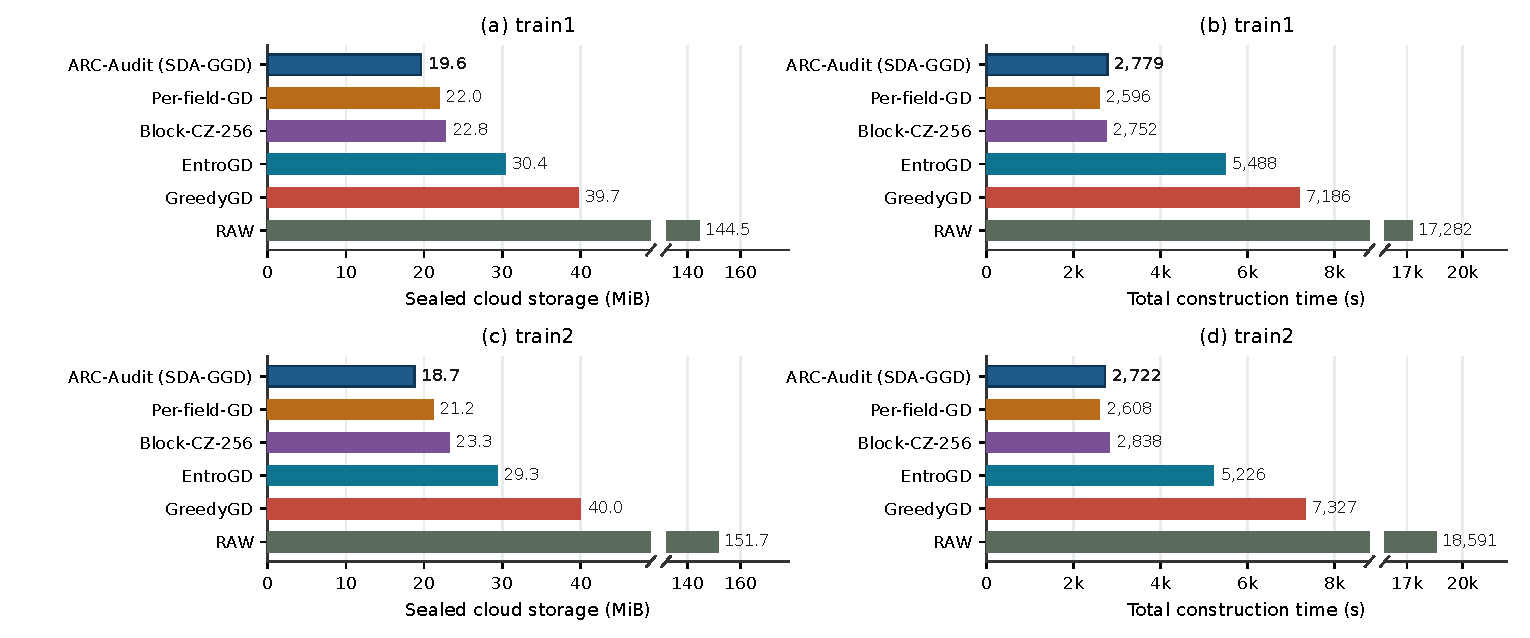
\includegraphics[width=0.90\textwidth]{figures/c1_arc_audit.pdf}
\caption{Full-dataset sealed cloud storage and total construction time of ARC-Audit (SDA-GGD) against internal and published GD baselines across all seven daily batches (RQ1). Broken horizontal axes preserve linear readability across deduplicated schemes and RAW.}
\label{fig:key-c1}\end{figure*}

\subsection{RQ1: Storage and Secure Construction}
Cross-field grouping achieves the lowest sealed cloud storage across all seven daily batches (Fig.~\ref{fig:key-c1}, Table~\ref{tab:rq1-ext}) while shifting moderate codec work and base state to the owner. SDA-GGD compresses sealed cloud storage to 19.601 MiB and 18.738 MiB, saving 10.79\%/11.44\% over Per-field-GD, 13.90\%/19.43\% over Block-CZ-256, 35.49\%/36.11\% over EntroGD~\cite{Zhao2026EntroGD}, and 50.63\%/53.21\% over GreedyGD~\cite{Hurst2024GreedyGD} (versus 144.46/151.70 MiB for RAW). Because per-page BLS12-381 tagging dominates sealing time, producing fewer ciphertext pages makes SDA-GGD's total build time (2,778.9/2,722.4 s) 49.36\%/47.91\% faster than EntroGD and 61.33\%/62.84\% faster than GreedyGD, despite higher codec time (533.5/528.2 s) and owner base state (3,206.7/2,723.4 KiB). All 84 daily builds pass decryption and ledger checks. The six-hour full-window check exhibits the same trade-off: SDA-GGD cuts cloud storage by 13.45\%/8.70\% over Per-field-GD (1.815/1.688 MiB vs.\ 2.097/1.849 MiB) with 18.50\%/14.29\% higher total build time and 328.0/210.6 KiB of owner state (all 16 builds pass).

\begin{table}[t]\centering\scriptsize
\caption{FULL-DATASET SEALED STORAGE AND CONSTRUCTION COST (RQ1, 7 DAILY BATCHES)}\label{tab:rq1-ext}
\setlength{\tabcolsep}{2.4pt}
\begin{tabular}{@{}llrrrrr@{}}\toprule
Seg. & Method & Cloud (MiB) & Owner (KiB) & Codec (s) & Tag (s) & Total (s)\\\midrule
t1 & \textbf{SDA-GGD} & \textbf{19.601} & 3,206.7 & 533.5 & 2,244.4 & \textbf{2,778.9}\\
 & Per-field-GD & 21.973 & 1,755.4 & 11.8 & 2,583.1 & 2,595.8\\
 & Block-CZ-256 & 22.765 & 0.70 & 0.31 & 2,750.6 & 2,751.9\\
 & EntroGD~\cite{Zhao2026EntroGD} & 30.385 & 0.69 & 13.7 & 5,472.7 & 5,488.0\\
 & GreedyGD~\cite{Hurst2024GreedyGD} & 39.703 & 0.69 & 90.1 & 7,093.9 & 7,185.8\\
 & RAW & 144.458 & 0.68 & 0.15 & 17,280.6 & 17,282.2\\\midrule
t2 & \textbf{SDA-GGD} & \textbf{18.738} & 2,723.4 & 528.2 & 2,193.0 & \textbf{2,722.4}\\
 & Per-field-GD & 21.159 & 1,742.4 & 12.0 & 2,594.9 & 2,608.1\\
 & Block-CZ-256 & 23.256 & 0.94 & 0.32 & 2,836.3 & 2,837.9\\
 & EntroGD~\cite{Zhao2026EntroGD} & 29.327 & 0.92 & 11.5 & 5,212.5 & 5,226.1\\
 & GreedyGD~\cite{Hurst2024GreedyGD} & 40.050 & 0.92 & 102.7 & 7,222.3 & 7,327.0\\
 & RAW & 151.702 & 0.90 & 0.16 & 18,588.7 & 18,590.7\\\bottomrule
\end{tabular}
\tabnote{t1/t2 denote \texttt{train1} (3 days, 216,001 rows) and \texttt{train2} (4 days, 226,801 rows). Values sum per-day medians (2 builds/day) under identical \texttt{py-ecc} BLS12-381 sealing.}
\end{table}

\begin{figure*}[t]\centering
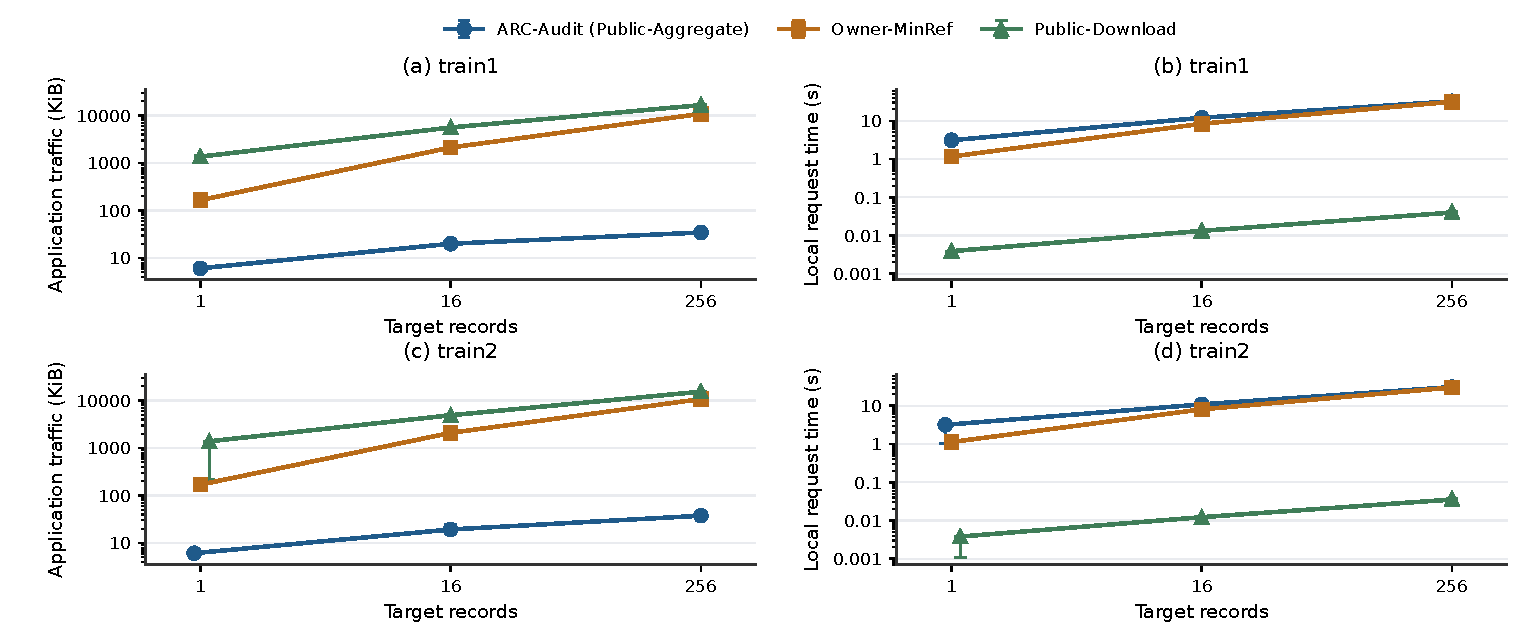
\includegraphics[width=0.90\textwidth]{figures/c2_arc_audit.pdf}
\caption{Application traffic per request and local processing time with reused contexts (RQ2). Application traffic includes declarations, challenges, any first-stage material, and the final response. The break-even link rates reported in the text use a simple serial-transfer estimate.}
\label{fig:key-c2}\end{figure*}

\subsection{RQ2: Public Audit Communication and Computation}
\emph{Internal interface trade-offs.}
Over the same public closure, proof aggregation cuts application traffic by over two orders of magnitude at the cost of local pairing verification (Fig.~\ref{fig:key-c2}). At $r{=}256$, Public-Aggregate transfers 34.58/37.62 KiB in 32.53/30.91 s locally, compared with 16.25/15.03 MiB in 0.040/0.035 s for Public-Download (break-even serial link rates of 4.19/4.07 Mbit/s). Relative to authorized Owner-MinRef, which transfers 10.65/10.50 MiB in total (10.61/10.46 MiB of first-stage references) to narrow dictionary coverage, Public-Aggregate cuts total traffic by 99.68\%/99.65\% while adding only 3.17\%/2.52\% local time (31.53/30.15 s for Owner-MinRef). At $r{=}1$, exact reference discovery saves pairing work (1.16/1.13 s vs.\ 3.11/3.17 s) at $\sim 27\times$ higher traffic (165.6/169.6 KiB vs.\ 6.09/6.11 KiB), but cross-target overlap steadily closes this latency gap as $r$ grows. Both aggregate interfaces return a constant 4,310 B proof per batch; cold context setup takes 8.10/7.81 s at $r{=}1$ and 20.82/21.17 s at $r{=}256$ (fetching 1.60/1.55 MiB of manifests and public parameters), and all 54 honest requests pass verification.

\emph{Mechanism controls.}
Table~\ref{tab:c2-mechanisms} isolates read reuse, aggregation, and data representation on two 16-target requests. Union planning matches cached traversal by reading each selected object once ($7\times$ fewer reads than uncached traversal). Aggregation shrinks proof size by $>125\times$ and verification time by $>68\times$ while rejecting mutated ciphertexts, and SDA-GGD reduces selected pages and local runtime relative to Per-field-GD under the same 4,310 B proof.

\begin{table}[t]\centering\small
\caption{AUDIT MECHANISM CONTROLS FOR TWO 16-TARGET REQUESTS (RQ2)}
\label{tab:c2-mechanisms}
\setlength{\tabcolsep}{3.2pt}
\begin{tabular}{@{}lrrrr@{}}\toprule
 & \multicolumn{2}{c}{train1} & \multicolumn{2}{c}{train2}\\
\cmidrule(lr){2-3}\cmidrule(l){4-5}
Traversal & Reads & Bytes & Reads & Bytes\\\midrule
Per-record & 5,643 & 23,113,728 & 892 & 3,651,221\\
Per-record, cached & 805 & 3,297,280 & 125 & 509,589\\
Union & 805 & 3,297,280 & 125 & 509,589\\\midrule
Proof format & Bytes & Verify (s) & Bytes & Verify (s)\\\midrule
Individual & 3,475,990 & 472.659 & 539,750 & 73.646\\
Aggregate & 4,310 & 3.477 & 4,310 & 1.074\\\midrule
Representation & Pages & Local (s) & Pages & Local (s)\\\midrule
Per-field-GD & 883 & 7.023 & 143 & 1.683\\
SDA-GGD & 805 & 6.437 & 125 & 1.489\\\bottomrule
\end{tabular}
\tabnote{Per-record traversal without caching counts repeated reads. For the representation comparison, SDA-GGD reads the bytes shown in the Union row, and Per-field-GD reads 3,616,768 B on train1 and 585,227 B on train2.}
\end{table}

\begin{figure*}[t]\centering
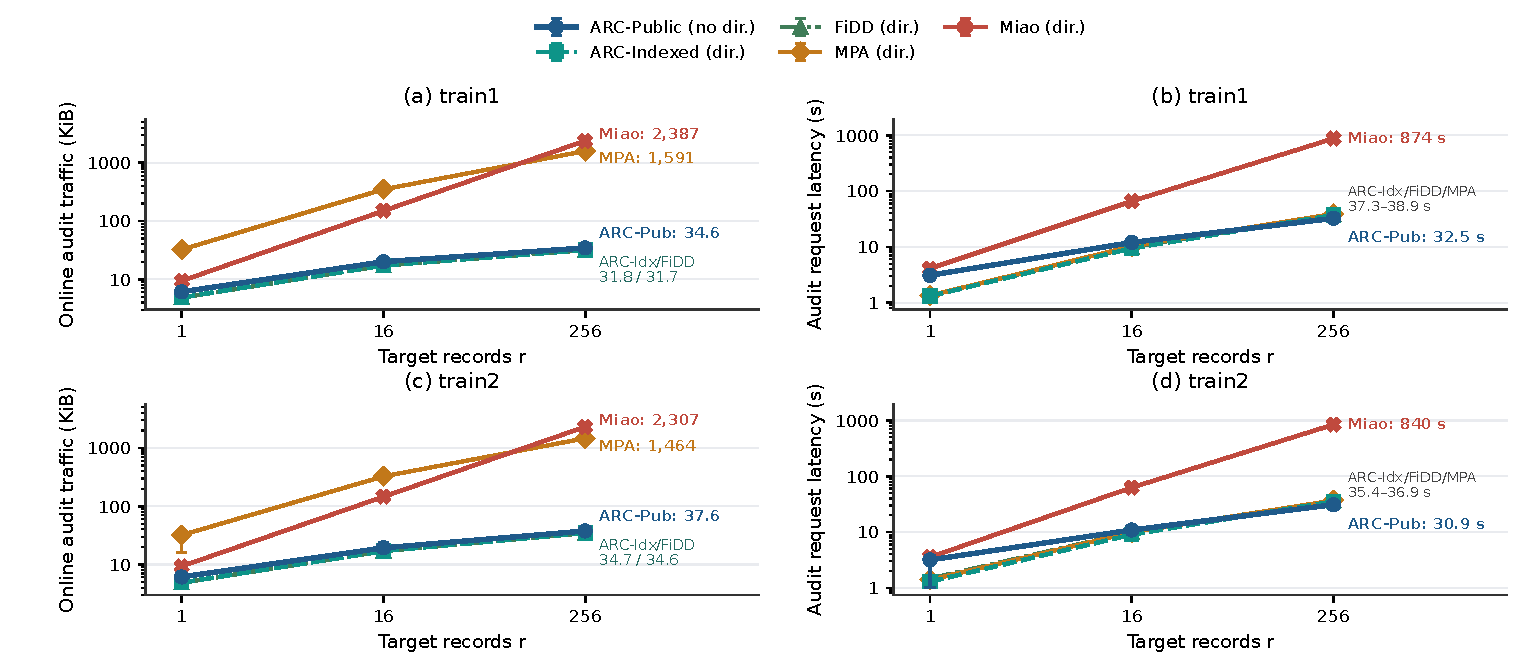
\includegraphics[width=0.90\textwidth]{figures/c2_ext_audit.pdf}
\caption{Full-dataset online audit traffic and request latency against published auditing schemes under the unified \texttt{py-ecc} BLS12-381 backend (RQ2). Error bars show observed min--max ranges across three matched target cohorts per $(segment,r)$. External schemes and \texttt{ARC-Indexed} rely on a 1,035.6 MiB owner-provisioned directory excluded from online traffic, whereas \texttt{ARC-Public} requires no directory.}
\label{fig:ext-c2}\end{figure*}

\emph{Comparison with published auditing schemes.}
Fig.~\ref{fig:ext-c2} and Table~\ref{tab:rq2-ext} compare ARC-Audit against FiDD~\cite{Huang2026FiDD}, MPA~\cite{Xu2026MPA}, and Miao~\cite{Miao2025} across all 18 cohorts. Over identical owner-indexed page sets, \texttt{ARC-Indexed} matches FiDD's compact online traffic (31.84/34.73 KiB vs.\ 31.70/34.56 KiB at $r{=}256$) with the lowest median latency among the four directory-based schemes across all six $(segment,r)$ settings. By contrast, MPA's per-page Merkle and KZG openings inflate $r{=}256$ online traffic by 39$\times$--46$\times$, while Miao's keyword-batched proofs inflate traffic by 61$\times$--69$\times$ and latency by 23$\times$. Crucially, \texttt{ARC-Public} eliminates the 1,035.6 MiB owner directory required by all three external schemes (plus Miao's 1,846.8 MiB persisted state, including a 1,765.8 MiB inverted index, and 4,556.7/5,307.1 s setup times for FiDD/Miao vs.\ 56.7 s for MPA) for only $\sim 9\%$ extra traffic. Finally, running the identical BLS12-381 proving and verification equations in native Rust \texttt{blst} lowers $r{=}256$ prover-plus-verifier computation from 34.77/32.71 s in a matched \texttt{py-ecc} microbenchmark to 100.81/100.79 ms (a 324.5$\times$--344.9$\times$ speedup).

\begin{table}[t]\centering\scriptsize
\caption{FULL-DATASET AUDIT COMPARISON AGAINST PUBLISHED SCHEMES (RQ2, \texttt{py-ecc} BLS12-381)}\label{tab:rq2-ext}
\setlength{\tabcolsep}{2.6pt}
\begin{tabular}{@{}lcccc@{}}\toprule
Method & $r$ & Pages (t1/t2) & Wire KiB (t1/t2) & Latency s (t1/t2)\\\midrule
\textbf{ARC-Public (no dir.)} & 1 & 340/345 & 6.09/6.11 & 3.11/3.17\\
ARC-Indexed & 1 & 79/78 & 4.88/4.87 & 1.32/1.29\\
FiDD~\cite{Huang2026FiDD} & 1 & 79/78 & 4.84/4.83 & 1.35/1.47\\
MPA~\cite{Xu2026MPA} & 1 & 79/78 & 32.31/31.90 & 1.35/1.40\\
Miao~\cite{Miao2025} & 1 & 79/78 & 9.38/9.31 & 4.10/3.55\\\midrule
\textbf{ARC-Public (no dir.)} & 256 & 4,143/3,830 & 34.58/37.62 & \textbf{32.53/30.91}\\
ARC-Indexed & 256 & 4,006/3,720 & 31.84/34.73 & 37.26/35.43\\
FiDD~\cite{Huang2026FiDD} & 256 & 4,006/3,720 & 31.70/34.56 & 37.86/36.69\\
MPA~\cite{Xu2026MPA} & 256 & 4,006/3,720 & 1,591.1/1,463.5 & 38.90/36.85\\
Miao~\cite{Miao2025} & 256 & 4,006/3,720 & 2,387.3/2,307.5 & 873.8/840.0\\\bottomrule
\end{tabular}
\tabnote{Medians over 3 matched full-dataset cohorts per $(segment,r)$ (t1/t2: \texttt{train1}/\texttt{train2}; intermediate $r{=}16$ curves are plotted in Fig.~\ref{fig:ext-c2}). External schemes and ARC-Indexed share a 1,035.6 MiB owner directory excluded from online traffic; ARC-Public ran standalone whereas directory-based baselines executed concurrently across dedicated cores (accounting for the $\sim 14\%$ timing offset at $r{=}256$). Native Rust \texttt{blst} lowers ARC-Audit $r{=}256$ total time to 100.81/100.79 ms.}
\end{table}

\begin{figure*}[t]\centering
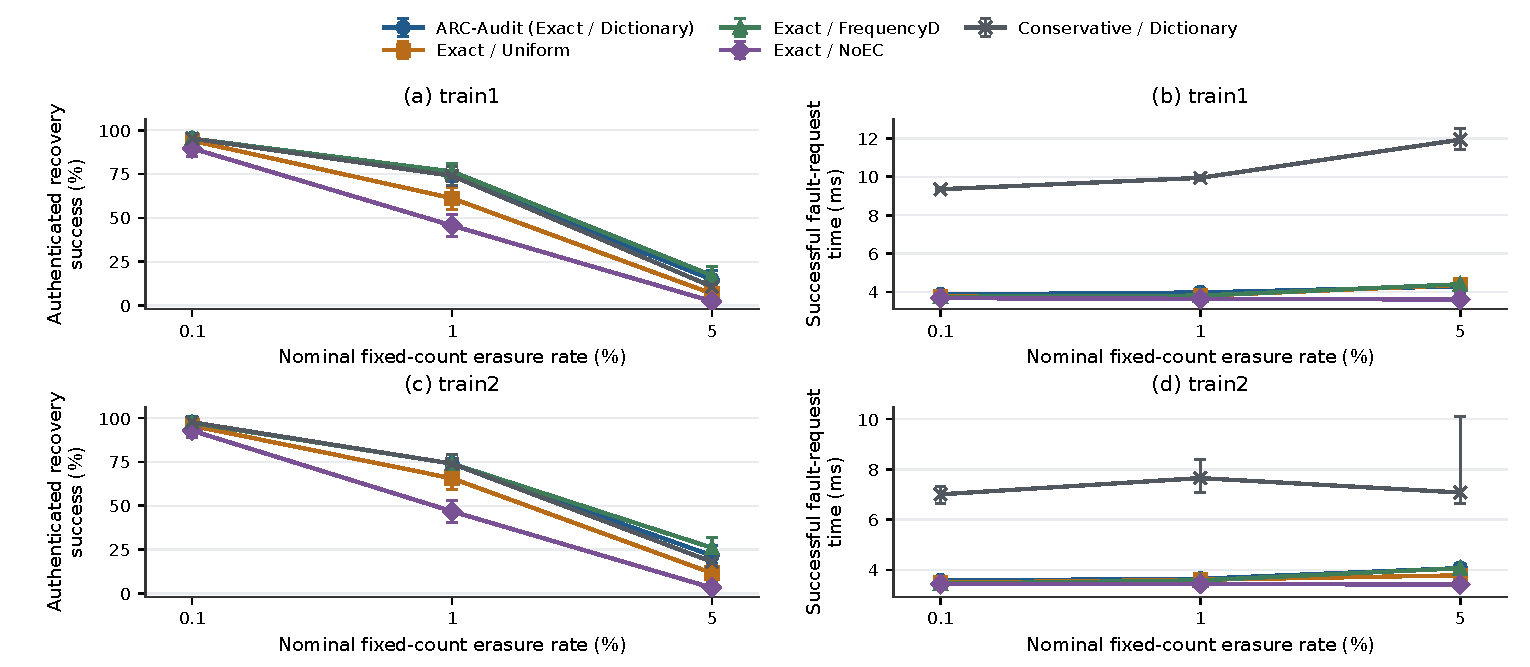
\includegraphics[width=0.90\textwidth]{figures/c3_arc_audit.pdf}
\caption{Authenticated recovery under erasures ($\beta{=}0.10$, RQ3). Left panels show recovery success with pointwise 95\% Wilson CIs ($N{=}250$); right panels show success-only median recovery time (excluding sidecar initialization) with 95\% bootstrap intervals. The remaining three Conservative controls are omitted for clarity.}
\label{fig:key-c3}\end{figure*}

\subsection{RQ3: Authenticated Recovery and Protection Allocation}
\emph{Protection placement and dependency selection.}
Under the 10\% budget cap, prioritizing shared dictionary pages consistently outperforms uniform redundancy (Fig.~\ref{fig:key-c3}). With Exact recovery at $\alpha{=}0.01$, Dictionary reaches 74.0\% on both segments versus 61.2\%/65.6\% for Uniform (+12.8/+8.4 pp) and 45.6\%/46.8\% for NoEC (at $\alpha{=}0.001$, Dictionary reaches 95.2\%/97.6\% vs.\ 94.0\%/95.6\% for Uniform). Ranking pages by reference-workload frequency (FrequencyD) already edges out Dictionary on \texttt{train1} at $\alpha{=}0.01$ (76.4\% vs.\ 74.0\%, tying at 74.0\% on \texttt{train2}) and provides a further gain at $\alpha{=}0.05$ (17.2\%/26.0\% vs.\ 14.8\%/21.6\%, per-layout differences $-2$ to $+8$ pp and $0$ to $+12$ pp). Holding Dictionary protection fixed at $\alpha{=}0.05$, Exact recovers every Conservative target plus +4.0/+3.6 pp (14.8\%/21.6\% vs.\ 10.8\%/18.0%) whenever only unreferenced dictionary pages are erased. Because Exact fetches fewer authenticated bytes, it also lowers clean recovery latency by $>2\times$ (3.69/3.51 ms vs.\ 8.99/7.21 ms) and reduces 5\%-loss latency for both successful (4.30/4.07 ms vs.\ 11.93/7.08 ms; Conservative's slight dip on \texttt{train2} reflects survivorship bias toward smaller daily batches) and failed requests (0.41/0.46 ms vs.\ 5.81/3.89 ms).

\begin{figure*}[t]\centering
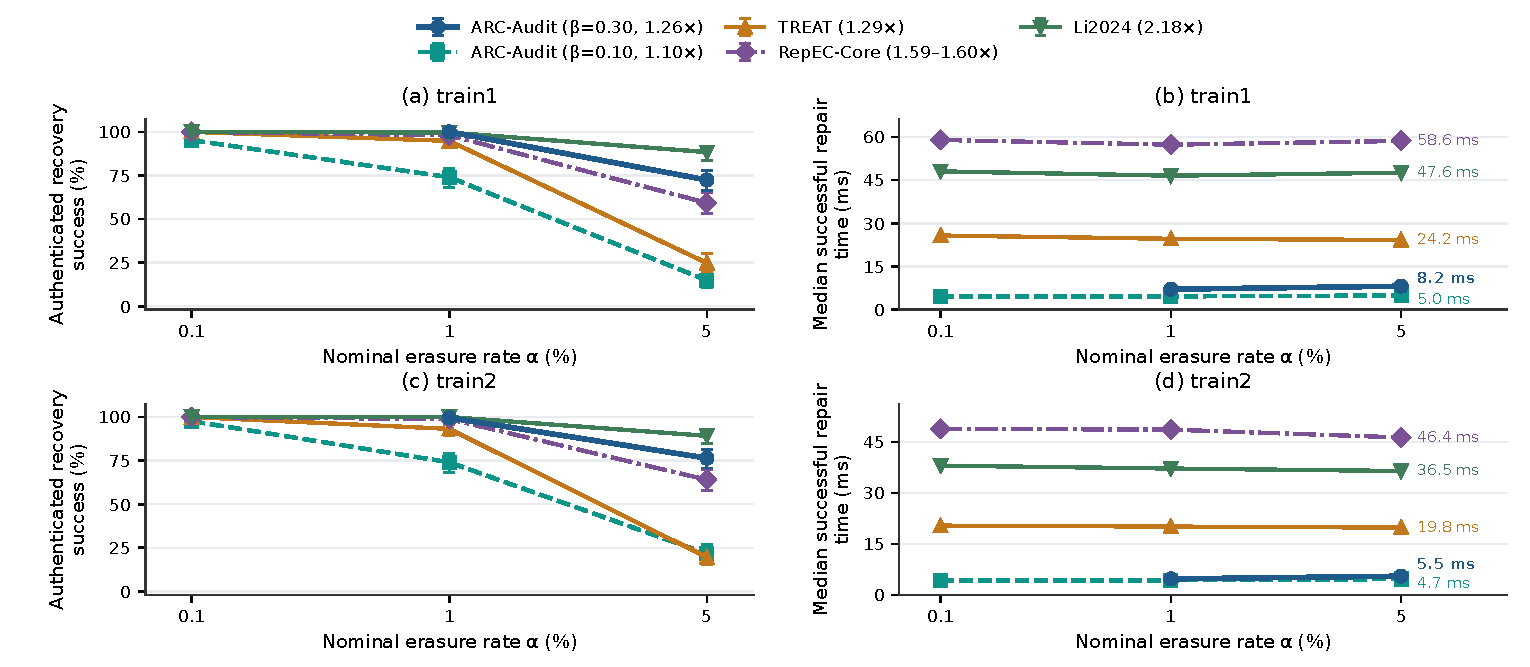
\includegraphics[width=0.90\textwidth]{figures/c3_ext_recovery.pdf}
\caption{Full-dataset selective recovery comparison against published shared-storage schemes across $N{=}250$ matched fault cases per point (RQ3). Left panels (a), (c) show authenticated recovery success with pointwise 95\% Wilson confidence intervals; right panels (b), (d) show median successful repair time (timing boundaries detailed in Table~\ref{tab:rq3-ext}). Legend labels report actual native storage ratios.}
\label{fig:ext-c3}\end{figure*}

\emph{Comparison with published recovery schemes.}
Fig.~\ref{fig:ext-c3} and Table~\ref{tab:rq3-ext} compare ARC-Audit ($\beta{=}0.10$ at $1.10\times$ and full-coverage $\beta{=}0.30$ at $1.26\times$) against TREAT~\cite{Taurone2024TREAT} ($1.29\times$), RepEC-Core~\cite{Zuo2022RepECPlus} ($1.59$--$1.60\times$), and Li2024~\cite{Li2024TNSE} ($2.18\times$); all 180 clean and 4,500 fault external outcomes (4,680 total) pass canonical-equality verification. At nearly equal storage ($1.26\times$ vs.\ $1.29\times$), ARC-Audit ($\beta{=}0.30$) outperforms TREAT by +5.2/+6.4 pp at $\alpha{=}0.01$ (100.0\%/99.6\% vs.\ 94.8\%/93.2\%) and by +47.6/+56.8 pp at $\alpha{=}0.05$ (72.4\%/76.4\% vs.\ 24.8\%/19.6\%), with 3.0$\times$--3.6$\times$ lower repair latency at $\alpha{=}0.05$ (3.5$\times$--4.3$\times$ at $\alpha{=}0.01$) and without TREAT's 1.2--1.4 MiB RLNC fragment downloads. It also strictly Pareto-dominates RepEC-Core at $\alpha{=}0.05$ (+13.2/+12.4 pp recovery with 21\% less storage and 7.2$\times$--8.4$\times$ faster repair). Li2024 attains the highest survival at $\alpha{=}0.05$ (88.4\%/89.2%), but incurs $2.18\times$ storage, $\sim 2\times$ download volume, and 36.5--48.0 ms repair latency.

\begin{table}[t]\centering\scriptsize
\caption{FULL-DATASET SELECTIVE RECOVERY AGAINST PUBLISHED SCHEMES (RQ3, $N{=}250$ CASES/POINT)}\label{tab:rq3-ext}
\setlength{\tabcolsep}{2.0pt}
\begin{tabular}{@{}lcccc@{}}\toprule
Method (Ratio) & $\alpha$ & Succ.\ \% (t1/t2) & Rep.\ ms (t1/t2) & DL KiB (t1/t2)\\\midrule
ARC $\beta{=}0.10$ ($1.10\times$) & 0.01 & 74.0/74.0 & 4.65/4.31 & 320/312\\
\textbf{ARC $\beta{=}0.30$ ($1.26\times$)} & 0.01 & \textbf{100.0/99.6} & \textbf{7.12/4.71} & --\\
TREAT~\cite{Taurone2024TREAT} ($1.29\times$) & 0.01 & 94.8/93.2 & 24.64/20.13 & 1,360/1,280\\
RepEC~\cite{Zuo2022RepECPlus} ($1.59$--$1.60\times$) & 0.01 & 98.0/98.8 & 57.30/48.68 & 320/308\\
Li2024~\cite{Li2024TNSE} ($2.18\times$) & 0.01 & 99.6/100.0 & 46.54/37.23 & 627/607\\\midrule
ARC $\beta{=}0.10$ ($1.10\times$) & 0.05 & 14.8/21.6 & 4.96/4.68 & 356/338\\
\textbf{ARC $\beta{=}0.30$ ($1.26\times$)} & 0.05 & \textbf{72.4/76.4} & \textbf{8.19/5.53} & --\\
TREAT~\cite{Taurone2024TREAT} ($1.29\times$) & 0.05 & 24.8/19.6 & 24.23/19.83 & 1,324/1,216\\
RepEC~\cite{Zuo2022RepECPlus} ($1.59$--$1.60\times$) & 0.05 & 59.2/64.0 & 58.64/46.37 & 336/320\\
Li2024~\cite{Li2024TNSE} ($2.18\times$) & 0.05 & 88.4/89.2 & 47.59/36.50 & 602/582\\\bottomrule
\end{tabular}
\tabnote{t1/t2: \texttt{train1}/\texttt{train2}; ARC/RepEC: ARC-Audit/RepEC-Core. At $\alpha{=}0.001$, all three external schemes reach 100.0\% and ARC $\beta{=}0.10$ reaches 95.2\%/97.6\%. Repair times for ARC $\beta{=}0.10$ and the three external schemes include reader and sidecar initialization (+0.6--0.75 ms over Fig.~\ref{fig:key-c3} for ARC $\beta{=}0.10$). Entries for ARC $\beta{=}0.30$ (100\% RS(10,8) coverage at $1.26\times$ storage; download volume omitted) are measured in the unconstrained-core budget evaluation excluding sidecar initialization, under which $\beta{=}0.10$ measures 7.19/7.63 ms on \texttt{train1} and 4.73/5.07 ms on \texttt{train2}.}
\end{table}

Taken together, protection allocation determines which objects receive redundancy and dependency selection determines which objects a request requires. Reducing the required page set under fixed protection and verification rules therefore enables more requests to complete within the tested HAI workloads and erasure settings.

\section{Conclusion and Future Work}
ARC-Audit uses a single authenticated layout to reconcile public auditing and authorized recovery over shared-compressed IIoT records. Without decryption keys, a public verifier builds a sufficient closure covering all dictionary pages a target set could reference and binds it to a fresh aggregate challenge. With decryption keys, an authorized retriever authenticates references first to narrow retrieval to exact dependencies, while verifying repaired and directly fetched ciphertexts under identical integrity rules.

Across two full HAI segments, ARC-Audit's grouped representation reduced sealed cloud storage by 10.79\% and 11.44\% relative to per-field GD and by 35.5\%--53.2\% relative to GreedyGD and EntroGD across all seven daily batches, while public aggregation substantially reduced application traffic over the same closure and cut online audit traffic by 39$\times$--69$\times$ relative to MPA and Miao without maintaining a gigabyte-scale external directory. Under 5\% nominal erasure and fixed dictionary-first protection, exact dependency resolution increased complete-record recovery over conservative closure retrieval by 4.0 and 3.6 percentage points whenever unreferenced dictionary pages were lost, and full-coverage ARC-Audit ($1.26\times$) outperformed TREAT ($1.29\times$) and RepEC-Core ($1.59$--$1.60\times$) by 47.6--56.8 and 12.4--13.2 percentage points.

Several directions remain open for future work. First, ARC-Audit currently seals immutable daily batches independently; extending the authenticated dependency map to support dynamic record appends, cross-batch dictionary reuse, and versioned manifest chains will require quantifying how page sharing affects manifest and index update costs. Second, because full batch manifests scale linearly with page count (1.55--1.60 MiB across the multi-day HAI segments), introducing Merkle-authenticated manifest slicing would allow memory-constrained edge verifiers to validate target closures on demand without caching complete descriptors. Third, evaluating recovery survival and repair read amplification under correlated node, rack, or whole-batch failures---alongside workload-adaptive or cross-stripe coding beyond fixed per-batch RS$(10,8)$---will better reflect large-scale cloud outage patterns. Finally, validating these trade-offs across additional heterogeneous IIoT datasets and integrating oblivious or padded retrieval to obscure authorized BaseID-driven page-access traces represent promising steps toward broader production deployment.

\bibliographystyle{IEEEtran}
\bibliography{IEEEabrv,bstcontrol,references}
\end{document}

